%% if some package prevents compilation, remove it

\documentclass[a4paper, 10pt]{article}
\usepackage{fullpage}
\usepackage{titling}
\usepackage{graphicx}
\usepackage{xcolor}
\usepackage{amsmath}
\usepackage{amssymb}
\usepackage{amsthm}
\usepackage{hyperref}
\usepackage{IEEEtrantools} 
\usepackage{bbm}
\usepackage{lineno}
\usepackage{multirow}
\usepackage{longtable}
\usepackage{makecell}
\usepackage{lipsum}
\usepackage{etoolbox} %% <- for \pretocmd and \apptocmd
\usepackage{algorithm}
\usepackage[noend]{algpseudocode}

\setlength{\droptitle}{-6em}   % This is your set screw, for shifting up the title
\renewcommand{\baselinestretch}{1.1}
\setlength{\parskip}{0.5em}

\author{Shivam and Sharan
  \\ September 2021}
\date{}
\title{FMA-PG Notes}

\makeatletter %% <- make @ usable in macro names
\newcommand*\linenomathpatch{\@ifstar{\linenomathpatch@AMS}{\linenomathpatch@}}
\newcommand*\linenomathpatch@[1]{
  \expandafter\pretocmd\csname #1\endcsname {\linenomathWithnumbers}{}{}
  \expandafter\pretocmd\csname #1*\endcsname{\linenomathWithnumbers}{}{}
  \expandafter\apptocmd\csname end#1\endcsname {\endlinenomath}{}{}
  \expandafter\apptocmd\csname end#1*\endcsname{\endlinenomath}{}{}
}
\newcommand*\linenomathpatch@AMS[1]{
  \expandafter\pretocmd\csname #1\endcsname {\linenomathWithnumbersAMS}{}{}
  \expandafter\pretocmd\csname #1*\endcsname{\linenomathWithnumbersAMS}{}{}
  \expandafter\apptocmd\csname end#1\endcsname {\endlinenomath}{}{}
  \expandafter\apptocmd\csname end#1*\endcsname{\endlinenomath}{}{}
}
\let\linenomathWithnumbersAMS\linenomathWithnumbers
\patchcmd\linenomathWithnumbersAMS{\advance\postdisplaypenalty\linenopenalty}{}{}{}
\makeatother %% revert @
\linenomathpatch{IEEEeqnarray}
\linenomathpatch{equation}
\linenomathpatch*{gather}
\linenomathpatch*{multline}
\linenomathpatch*{align}
\linenomathpatch*{alignat}
\linenomathpatch*{flalign}

\DeclareMathOperator{\E}{\mathbb{E}}

\begin{document}
\maketitle
\vspace{-2cm}
% \linenumbers

\section{Experiments in the tabular setting} \label{app:tabular_experiments}
In this section\footnote{The code implementation for the algorithms and the environment corresponding to experiments presented in this section is available at \url{https://github.com/svmgrg/fma-pg}.}, we study the performance of four different policy gradient (PG) algorithms. Two of these can be directly obtained from the FMA-PG framework: sMDPO (FMA-PG with a softmax policy and log-sum-exp mirror map; see Eq. \ref{eq:fmd-softmax-kl-practical} in the main text) and MDPO (FMA-PG with direct parameterization and a negative entropy mirror map; see Eq. \ref{eq:fmd-softmax-statewise} in the main text). And the other two are the existing popular PG algorithms: TRPO and PPO. 

Further, to better understand the reason behind the performance of each of these methods, in addition to studying the objective functions used by these PG algorithms, we will also consider the impact of the optimization techqniques used to implement them. In particular, we will look at three different variants of sMDPO, MDPO, and TRPO based on whether they use a regularized objective with a fixed stepsize (similar to the conventional sMDPO and MDPO), a regularized objective with Armijo line search, or a constrained objective with line search (similar to the conventional TRPO). 

\subsection{Algorithmic Details} \label{sec:tabular_algorithmic_details}
We begin by specifying the different PG objectives used by the algorithms and the two optimization procedures we use for maximizing these objectives. The sMDPO and MDPO algorithms motivated by the FMA-PG framework can be considered as regularized algorithms, which can be summarized by
\begin{equation}
  \max_\theta \; \mathcal{J}_{\text{PG-Alg}} - \frac{1}{\eta} \mathcal{C}_{\text{PG-Alg}}, \label{eq:regularized_program}
\end{equation}
where the terms $\mathcal{J}_{\text{PG-Alg}}$ and $\mathcal{C}_{\text{PG-Alg}}$ are given in Table \ref{table: ablation_study}. One way of solving this objective is by gradient descent using a fixed stepsize $\alpha$, as specified in Algorithm \ref{alg:generic}; we call this setting as \texttt{Regularized+fixed_stepsize}. We can equivalently solve such an unconstrained optimization problem by using an Armijo-style backtracking line search, which we call as \texttt{Regularized+line search}. Note that, we can use this same form to obtain a regularized version of the TRPO algorithm\footnote{For TRPO, this objective is almost the same as PPO with KL penalty (Eq. 8, \citet{schulman2017proximal}) except that PPO uses the advantage function and we used the action value function (which, as we discussed in the caption of Table \ref{table: ablation_study}, doesn't really matter). It is also similar to the objective stated in the TRPO paper (Section 4, \citet{schulman2015trust}) except that this has an average KL divergence instead of the max KL divergence given in the original paper.} as well.

  \begin{table}[!hbt]
  \centering
  \renewcommand{\arraystretch}{1.5}
  \renewcommand{\tabcolsep}{0.2cm}
  \begin{tabular}{c|l|c}
    \textbf{PG Alg.} & \hspace{2cm} \textbf{Objective} $(\mathcal{J})$ & \textbf{Constraint} $(\mathcal{C})$ \\
    \hline \hline
    sMDPO &
    $\sum_s d^{\pi_t}(s) \sum_a p^{\pi_t}(a | s) A^{\pi_t}(s, a) \log \frac{p^{\pi_\theta}(s, a)}{p^{\pi_t}(s, a)}$ &
    $\sum_s d^{\pi_t}(s) \cdot \text{KL}(p^{\pi_t}(\cdot | s) \| p^{\pi_\theta}(\cdot | s))$\\
    \hline
    TRPO &
    $\sum_s d^{\pi_t}(s) \sum_a p^{\pi_t}(a | s) Q^{\pi_t}(s, a) \frac{p^{\pi_\theta}(s, a)}{p^{\pi_t}(s, a)}$ &
    \texttt{(same as above)} \\
    \hline
    MDPO &
    $\sum_s d^{\pi_t}(s) \sum_a p^{\pi_t}(a | s) A^{\pi_t}(s, a) \frac{p^{\pi_\theta}(s, a)}{p^{\pi_t}(s, a)}$ &
    $\sum_s d^{\pi_t}(s) \cdot \text{KL}(p^{\pi_\theta}(\cdot | s) \| p^{\pi_t}(\cdot | s))$
  \end{tabular}
  
  \caption{The objectives and the constraints corresponding to the different PG algorithms. Note that the objective $\mathcal{J}$ for both TRPO and MDPO is essentially equivalent to each other, since maximizing either of them would lead to the same solution. The reason for this is that the difference between the two objectives is $\sum_s d^{\pi_t} V^{\pi_t}(s)$, which is independent of the policy weight $\theta$).} 
  \label{table: ablation_study}
\end{table}

On the other hand, the conventional TRPO algorithm instead solves a constrained optimization problem given by the equation
\begin{equation}
  \max_\theta \; \mathcal{J}_{\text{PG-Alg}} \quad \text{subject to } \quad \mathcal{C}_{\text{PG-Alg}} \leq \delta, \label{eq:constrained_program}
\end{equation}
with the terms $\mathcal{J}_{\text{PG-Alg}}$ and $\mathcal{C}_{\text{PG-Alg}}$ again given in Table \ref{table: ablation_study}. The regularized program of Eq. \ref{eq:regularized_program} can be considered a ``softer'' version of the constrained program of Eq. \ref{eq:constrained_program}. To solve the constrained optimization problem, we use the exact same process used by the TRPO paper \citep{schulman2015trust}: we use line search to find the maximal stepsize that increases the objective value in the direction of maximum ascent while satisfying the constraint; see Section \ref{app:trpo} for details. We call this setting as \texttt{Constrained+line search}. Further, using Eq. \ref{eq:constrained_program}, we can also obtained constrained versions of sMDPO and MDPO. 

The motivation behind considering these three different variants for sMDPO, MDPO, and TRPO is to figure out that how much of the performance difference between these algorithms comes from their exact objectives (Table \ref{table: ablation_study}) and how much of it comes from the optimization techniques employed. We also summarize the gradient of these objectives in Table \ref{table: ablation_study_grad}. The corresponding gradient derivations for the algorithms (including PPO) are presented in Appendix \ref{app:tabular_derivations}.

\begin{table}[!hbt]
  \centering
  \renewcommand{\arraystretch}{1.5}
  \renewcommand{\tabcolsep}{0.2cm}
  \begin{tabular}{c|l|c}
    \textbf{PG Alg.} & \hspace{1cm} \textbf{Grad. objective} $(\nabla_{\theta(s, a)} \mathcal{J})$ & \textbf{Grad. constraint} $(\nabla_{\theta(s, a)} \mathcal{C})$ \\
    \hline \hline
    sMDPO &
    $d^{\pi_t}(s) p^{\pi_t}(a|s) A^{\pi_t}(s, a)$ &
    $d^{\pi_t}(s) \left[ p^\pi(a | s) - p^{\pi_t}(a|s) \right]$ \\
    \hline
    TRPO &
    $d^{\pi_t}(s) p^\pi(a | s) \left[ Q^{\pi_t}(s, a) - \sum_b p^\pi(b | s) Q^{\pi_t}(s, b) \right]$ &
    \texttt{(same as above)} \\
    \hline
    MDPO &
    $d^{\pi_t}(s) p^\pi(a | s) \left[ A^{\pi_t}(s, a) - \sum_b p^\pi(b|s) A^{\pi_t}(s, b) \right]$ &
    $\begin{array}{c} d^{\pi_t}(s) p^\pi(a | s) \times \\ \left[ \log \frac{p^\pi(a | s)}{p^{\pi_t}(a | s)} - \text{KL}(p^\pi(\cdot | s) \| p^{\pi_t}(\cdot | s)) \right] \end{array}$
  \end{tabular}
  
  \caption{The gradients of the objectives and constraints w.r.t. the policy parameter corresponding to the different PG algorithms. Note that the gradient of the objective for both TRPO and MDPO is exactly equal to each other.}
  \label{table: ablation_study_grad}
\end{table}

\subsection{Empirical Details}
In all our tabular experiments, we assumed full access to the environment dynamics and used the analytically calculated expected gradient updates for all the algorithms, and therefore the results closely follow the theoretical properties of the PG methods. Doing so, essentially made this a study of the optimization properties of the four PG algorithms considered. We use a policy gradient agent with a tabular softmax policy parameterization, and evaluate the algorithms on two tabular episodic environments: CliffWorld (environment description and its properties are discussed in Figure \ref{fig: cliffworld}) and DeepSeaTreasure  (\citet{osband2019behaviour}; with $n=5$, discount factor $\gamma=0.9$, 25 different states, and two actions). 

\begin{figure}[h]
  \centering
  \includegraphics[scale=0.36]{cliffworld.pdf}
  \caption{The episodic CliffWorld environment and the learning curve for MDPO on it illustrating three different locally optimal policies. \textbf{(Left)} We consider a variant of the CliffWorld environment (Example 6.6, \citet{sutton18book}) containing 21 different states and four actions per state. The agent starts in the \texttt{Start} state and has four cardinal actions which deterministically move it into the corresponding next state. The objective is to reach the \texttt{Goal} state as quickly as possible. If the agent falls into a state marked by \texttt{Cliff}, any subsequent action taken by it moves it back to the start state and yields a reward of $-100$. Similarly, once in the goal state, any action takes the agent into the terminal state and yields a reward of $+1$. All the other transitions have zero reward and the discount factor is $\gamma = 0.9$. It is easy to see that the optimal policy will have a value of $v^*(s_0) = 0 + \gamma \cdot 0 + \cdots + \gamma^5 \cdot 0 + \gamma^6 \cdot 1 = 0.9^6 = 0.53$. \textbf{(Right)} We show the learning curve for the analytical MDPO update using $\eta = 1$. This curve shows three different locally optimal policies. We later show in our experiments, that the different PG agents often get stuck on one of these policies.}
  \label{fig: cliffworld}
 \end{figure}
  
\begin{figure*}[!tbp]
    \centering
    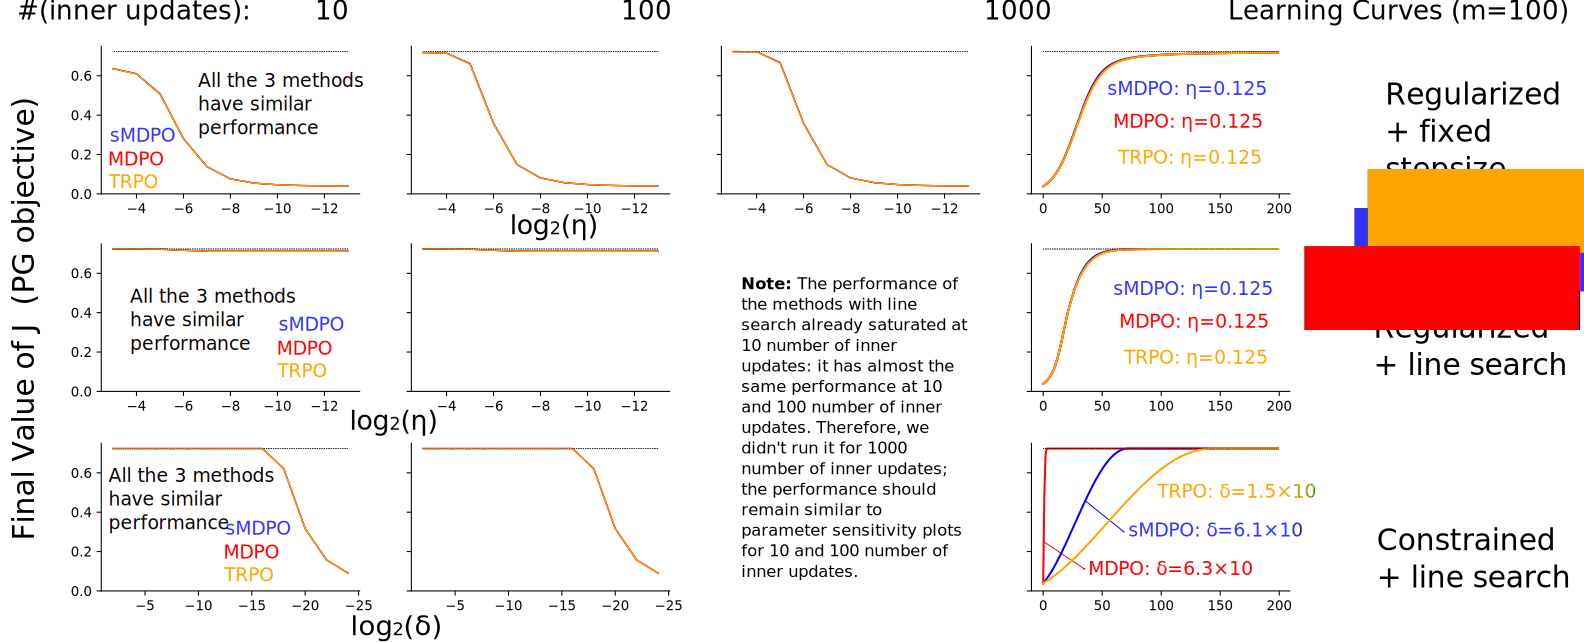
\includegraphics[width=0.9\textwidth]{deep_sea_treasure_ablation.pdf}
    \caption{The parameter sensitivity plots for the  PG algorithms on the DeepSeaTreasure environment for different number of inner loop updates. The $x$ axis shows sweep over one parameter of the corresponding PG algorithm. And for each point on the $x$-axis, we chose the best performing second parameter of the algorithm: the inner loop stepsize $\alpha$ for the first row, the Armijo constant for the second row, and there is no additional parameter for the last row. The faint black line near the top of each subplot depicts the value of the optimal policy. The last column shows the learning curves for the best performing parameter configuration for each method.
    \label{fig:dst_sensitivity_plots}}
\end{figure*}
 
\textbf{Hyperparameter configurations:} We trained each of the method for 2000 iterations for CliffWorld (200 iterations for DeepSeaTreasure). Each iteration consisted of multiple inner loop updates (we represent this number by $m$); these updates are performed in an off-policy fashion that is typical of all these algorithms (also see Algorithm \ref{alg:generic} in the main paper). We swept over the relevant parameters of the PG algorithms. For the \texttt{Regularized} variants (both with and without line search) of sMDPO, MDPO, and TRPO, this was $\eta \in \{2^{-13}, 2^{-12}, \ldots, 2^{-1}\}$. For \texttt{fixed stepsize} variant of  sMDPO, MDPO, TRPO, and PPO, we swept over the inner loop stepsize $\alpha \in \{2^{-13}, 2^{-12}, \ldots, 2^3\}$ for CliffWorld (and $\{2^{-13}, 2^{-12}, \ldots, 2^{-2}\}$ for DeepSeaTreasure). For PPO, we additionally considered the clipping parameter $\epsilon \in \{0.01, 0.1, 0.2, 0.3 \ldots, 0.8, 0.9, 0.99\}$. For the \texttt{Regularized+line search} variant of  sMDPO, MDPO, TRPO, we also considered different Armijo constant in the set $\{0.0, 0.1, 0.3, 0.5, 0.7, 0.9, 0.99\}$, and used a decay factor of 0.9, initialized the maximal stepsize to $10.0$ and used a warm-start factor of $2.0$. Finally, for the \texttt{Constrained+line search} variant of  sMDPO, MDPO, and TRPO, we swept over the trust region size $\delta \in \{2^{-24}, 2^{-22}, \ldots, 2^{-2}\}$, used a fixed backtracking decay parameter of 0.9, an analytically obtained maximal stepsize (see Appendix \ref{app:trpo}), and an Armijo constant of 0.0 (i.e. no Armijo line search).

\subsection{Experimental Results}
\textbf{Learning Curves:} We show the learning curves corresponding to the best performing hyperparameters for the four algorithms conventional sMDPO and MDPO (\texttt{Regularized+fixed_stepsize}), conventional TRPO (\texttt{Constrained+line search}), and PPO in Figure \ref{fig:learning_curves} (main paper). To select the hyperparameters for each setting, we ran sweeps over different configurations and chose the ones that resulted in the best final performance at the end of 2000 iterations for CliffWorld (and 200 iterations for DeepSeaTreasure). From this figure, we see that for CliffWorld, all the methods except PPO (PPO got stuck in a ``safe'' sub-optimal policy) are able to converge to the optimal policy, and TRPO has the fastest convergence (learned the optimal policy in less than 200 iterations). On the other hand for DeepSeaTreasure, we note that all the methods converge to the optimal policy with PPO having the fastest convergence and TRPO having the slowest convergence. Finally, we should also mention that the TRPO's update was the costliest (more than two times slower than the rest of the methods) in terms of wall time, likely because of the backtracking from the line-search. 

\textbf{Parameter Sensitivity and Ablation Study:} We show the final performance for sMDPO, MDPO, and TRPO in Figure \ref{fig:cliffworld_sensitivity_plots} (after 2000 iterations for CliffWorld; main paper) and Figure \ref{fig:dst_sensitivity_plots} (after 200 iterations for DeepSeaTreasure). The different rows correspond to the variants \texttt{Regularized+fixed_stepsize}, \texttt{Regularized+line search}, and \texttt{Constrained+line search} for each of the methods. And different columns correspond to different number of inner loop updates\footnote{For the \texttt{Constrained+line search} of each method, we observed that the performance saturated after $m = 10$; in particular the sensitivity plots are identical for $m=10$ and $m=100$. Therefore, the performance at $m=1000$ should be exactly equivalent to the performance given at $m=100$, and consequently we skipped running that experiment.}. The last column in each row shows the learning curves for the best performing parameter setting. The $x$-axis on each subplot of first two rows shows the regularization strength $\eta$. For the \texttt{Regularization + fixed stepsize} variant, we chose the best performing $\alpha$ for each $\eta$, and for \texttt{Regularization + line search} variant, we chose the best performing Armijo constant for each $\eta$. The last row (constrained variant) had only a single parameter, the trust region magnitude, $\delta$ that is shown on the $x$-axis.

From these figures, we see as the value of $m$ increased, the performance of  the fixed stepsize algorithms improved. We also note that adding line search to regularized methods improved their parameter sensitivity to a large extent. Although, for CliffWorld, none of the \texttt{Regularized+line search} variant were able to achieve the optimal policy. We believe that the reason for this is that with warm-start the algorithms started using very large stepsizes (as large as 1000), which lead to an early convergence to a locally optimal policy. To verify this further, we tried running these algorithms without warm start and a maximal stepsize of 1.0; this allowed the methods to achieve the optimal policy for a small range of $\eta$ values, but also made them much more sensitive different $\eta$s. For the constrained version, we see that all the three algorithms achieve the optimal policy and are generally insensitive to the $\delta$ values. This is likely because this variant uses the (near) optimal steepest ascent direction with the maximal stepsize, achieved via line search. Finally, we note that for DeepSeaTreasure, all the methods had essentially the same performance and achieved the optimal policy in each case; we attribute this to the simplicity of the environment coupled with access to true gradient updates.

We provide the sensitivity plot for PPO for the two environments in Figure \ref{fig:ppo_plots}. We again see that increasing the number of inner updates helps PPO achieve better performance on both the environments. We also note that for no value of the parameters we tested, did PPO achieve the optimal policy on CliffWorld.

\begin{figure*}[!tbp]
    \centering
    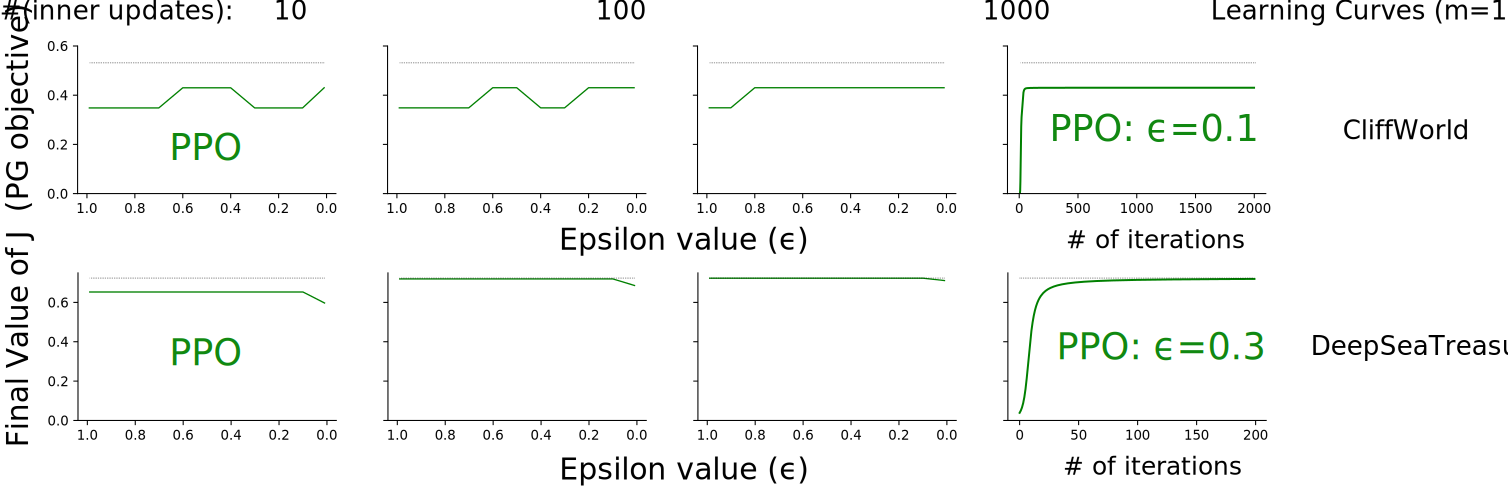
\includegraphics[width=0.9\textwidth]{ppo.pdf}
    \caption{The parameter sensitivity plots for PPO on the CliffWorld and DeepSeaTreasure environments for different number of inner loop updates. The $x$ axis shows sweep over the clipping parameter $\epsilon$. The curve shows the final performance of the method for the best performing inner loop stepsize $\alpha$ given the $\epsilon$ value.
    \label{fig:ppo_plots}}
\end{figure*}

\subsection{Discussion} \label{app:tabular_discussion}
These experiments served to demonstrate three major points:
\begin{enumerate}
\item The optimization methods might matter as much as the policy gradient objectives being considered. In particular, we found that much of TRPO's performance came from formalizing the optimization problem as a constrained program solved using the optimal descent direction and a large stepsize found using line search. Not only did TRPO's performance suffer when we replaced the constraint with regularization, the performance of both sMDPO and MDPO improved significantly when we used TRPO style optimization on their objectives. Additionally, we found that line search greatly improved the parameter sensitivity of all the algorithms.
\item We also note that the optimal $\eta$ values chosen by the \texttt{Regularized+fixed_stepsize} variants of sMDPO and MDPO were much larger than the values predicted by our theoretical results. For instance, the maximal $\eta$ values for CliffWorld are 
\begin{align*}
\eta_{\text{sMDPO}} &= \frac{1 - \gamma}{r_m - r_l} = \frac{1 - 0.9}{100 - (-1)} = 9.9 \times 10^{-4}, \\
\eta_{\text{MDPO}} &= \frac{(1 - \gamma)^{3}}{(r_m - r_l) \cdot 2\gamma |\mathcal{A}|} = \frac{(1 - 0.9)^{3}}{101 \times 2 \times 0.9 \times 4} = 1.4 \times 10^{-6}.
\end{align*}
And for DeepSeaTreasure, 
\begin{align*}
\eta_{\text{sMDPO}} &= \frac{1 - 0.9}{1 - (-0.01 / 5)} = 1.0 \times 10^{-2} \\
\eta_{\text{MDPO}} &= \frac{(1 - 0.9)^{3}}{(1 - (-0.01 / 5)) \times 2 \times 0.9 \times 2} = 2.8 \times 10^{-4}.
\end{align*}
Note that these values of $\eta$ are extremely small, and while the FMA-PG framework still guarantees policy improvement with these values, the convergence would be much slower. This is natural since these $\eta$ bounds are based on the smoothness of the policy objective $\mathcal{J}$ and such bounds are usually quite loose. Finally, also note that the optimal $\eta$ for sMDPO found by the experiments (in Figure \ref{fig:learning_curves}) is closer to that predicted by the theory, as compared to MDPO.
\item Each of the algorithms benefited from increasing the number of inner loop updates. These off-policy type of updates allow PG algorithms to ``maximally squeeze'' out all the information present in the data they have already collected, thereby allowing them to improve their performance without any additional interactions with the environment. This demonstrates the strength of these methods over simpler algorithms like REINFORCE \citep{williams1992simple} which only have a single update per batch of sampled data. 
\end{enumerate}

To conclude, our experiments suggest that FMA-PG provides general purpose surrogate functions with policy improvement guarantees, which when combined with existing optimization techniques can yield policy gradient algorithms that are competitive to existing state-of-the-art methods.

\newpage
\section{Analytical Updates and Gradient Expressions for tabular PG Algorithms} \label{app:tabular_derivations}
In the rest of this section, we give the calculations (the closed form analytical solutions for sMDPO and MDPO, and the gradient expressions for all four algorithms) employed in our implementation for tabular PG algorithms given in Appendix \ref{app:tabular_experiments}.

\subsection{sMDPO with Tabular Parameterization}
\subsubsection{Closed Form Update with Direct Representation}
Our goal is to find the closed form solution to the following optimization problem (from Eq. \ref{eq:fmd-softmax-kl-practical}, main paper):
\begin{equation}
  \pi_{t+1} = \arg\max_{\pi \in \Pi} \underbrace{\left[ \sum_s d^{\pi_t}(s) \sum_a p^{\pi_t}(a | s) \left(A^{\pi_t}(s, a) + \frac{1}{\eta} \right) \log \frac{p^\pi(s, a)}{p^{\pi_t}(s, a)} \right]}_{=: \ell^{\pi_t}_{\text{sMDPO}}}, \label{eq: optim_problem_sppo}
\end{equation}
subject to the constraints on policy $p^\pi$. We will solve this problem by assuming the policy $\pi \equiv p^\pi$ as an $|\mathcal{S}| \times |\mathcal{A}|$ table satisfying the standard constraints
\begin{align*}
  \sum_a p^\pi(a | s) &= 1,  \quad \forall s \in \mathcal{S} \\
  p^\pi(a | s) &\geq 0,  \quad \forall s \in \mathcal{S}, \; \forall a \in \mathcal{A}.
\end{align*}
We begin by formulating this problem using Lagrange multipliers $\{\lambda_s\}_{s \in \mathcal{S}}$ and $\{\lambda_{s, a}\}_{s, a \in \mathcal{S} \times \mathcal{A}}$ for all states $s$ and actions $a$:
\begin{align}
  \mathcal{L}(p^\pi, \lambda_s, \lambda_{s, a}) &= \sum_s d^{\pi_t}(s) \sum_a p^{\pi_t}(a | s) \left(A^{\pi_t}(s, a) + \frac{1}{\eta} \right) \log \frac{p^\pi(a | s)}{p^{\pi_t}(a | s)} \nonumber \\
  & \quad \; - \sum_{s, a} \lambda_{s, a} p^\pi(a | s) - \sum_s \lambda_{s} \bigg( \sum_a p^\pi(a | s) - 1 \bigg),
\end{align}
where we abused the notation, in $\mathcal{L}(p^\pi, \lambda_s, \lambda_{s, a})$, by using $\lambda_s$ to represent the set $\{\lambda_s\}_{s \in \mathcal{S}}$ and $\lambda_{s, a}$ to represent the set $\{\lambda_{s, a}\}_{s, a \in \mathcal{S} \times \mathcal{A}}$. The KKT conditions (Theorem 12.1, \citet{nocedal2006numerical}) for this constrained optimization problem can be written as:
\begin{align}
  \nabla_{p^\pi(b|x)} \mathcal{L}(p^\pi, \lambda_s, \lambda_{s, a}) &= 0, \quad \forall x \in \mathcal{S}, \; \forall b \in \mathcal{A} \tag{C1} \label{eq: KKT1} \\
  \sum_a p^\pi(a | s) &= 1, \quad \forall s \in \mathcal{S} \tag{C2} \label{eq: KKT2} \\
  p^\pi(a | s) &\geq 0, \quad \forall s \in \mathcal{S}, \; \forall a \in \mathcal{A} \tag{C3} \label{eq: KKT3} \\
  \lambda_s &\geq 0, \quad \forall s \in \mathcal{S} \tag{C4} \label{eq: KKT4} \\
  \lambda_{s} \bigg( \sum_a p^\pi(a | s) - 1 \bigg) &= 0, \quad \forall s \in \mathcal{S} \tag{C5} \label{eq: KKT5} \\
  \lambda_{s, a} p^\pi(a | s) &= 0, \quad \forall s \in \mathcal{S}, \; \forall a \in \mathcal{A}. \tag{C6} \label{eq: KKT6}
\end{align}

We now solve this system. Simplifying Eq. \ref{eq: KKT1} for an arbitrary state-action pair $(x, b)$ gives us:
\begin{align}
  \nabla_{p^\pi(b | x)} \mathcal{L}(p^\pi, \lambda_s, \lambda_{s, a}) &= d^{\pi_t}(x) p^{\pi_t}(b|x) \left( A^{\pi_t}(x, b) + \frac{1}{\eta} \right) \frac{1}{p^\pi(b|x)} - \lambda_{x, b} - \lambda_x = 0 \nonumber \\
  \Rightarrow \qquad \qquad \qquad \quad p^\pi(b | x) &= \frac{d^{\pi_t}(x) p^{\pi_t}(b|x) (1 + \eta A^{\pi_t}(x, b))}{\eta (\lambda_x + \lambda_{x, b})}. \label{eq: lagrangian_derivative_sppo}
\end{align}
Let us set 
\begin{equation}
  \lambda_{s, a} = 0, \quad \forall s \in \mathcal{S}, \; \forall a \in \mathcal{A}.
\end{equation}
Combining Eq. \ref{eq: lagrangian_derivative_sppo} with the second KKT condition gives us
\begin{equation}
  \lambda_s = \frac{1}{\eta} \sum_a d^{\pi_t}(s) p^{\pi_t}(a|s) (1 + \eta A^{\pi_t}(s, a)).
\end{equation}
Therefore, with the standard coverage assumption $d^{\pi_t}(s) > 0$, $p^\pi(a | s)$ becomes
\begin{equation}
  p^\pi(a | s) = \frac{p^{\pi_t}(a|s) (1 + \eta A^{\pi_t}(s, a))}{\sum_b p^{\pi_t}(b|s) (1 + \eta A^{\pi_t}(s, b))}.
\end{equation}
Note that $d^{\pi_t}(s), p^{\pi_t}(a|s) \geq 0$ for any state-action pair, since they are proper measures. We also need to ensure that
\begin{equation*}
  1 + \eta A^{\pi_t}(s, a) \geq 0
\end{equation*}
to satisfy the third and fourth KKT conditions. One straightforward way to achieve this is to define $p^\pi(a | s) = 0$ whenever $1 + \eta A^{\pi_t}(s, a) < 0$, and accordingly re-define $\lambda_s$. This gives us the final solution to our original optimization problem (Eq. \ref{eq: optim_problem_sppo}):
\begin{equation}
  \pi_{t+1} = p^\pi(s, a) = \frac{p^{\pi_t}(a|s) \max(1 + \eta A^{\pi_t}(s, a), 0)}{\sum_b p^{\pi_t}(b|s) \max(1 + \eta A^{\pi_t}(s, b), 0)}.
\end{equation}
However, it leaves us one last problem to deal with: Is it always true that given any state $s$, there always exists atleast one action $a$, such that $1 + \eta A^{\pi_t}(s, a) \geq 0$? Because otherwise, we would fail to satisfy the second KKT condition. But not that this is not a problem since we can put a condition on $\eta$ in order to fulfill this constraint.

\subsubsection{Gradient of the Loss Function with Softmax Policy Representation}
Consider the softmax policy representation
\begin{equation}
  p^\pi(b | x) = \frac{e^{\theta(x, b)}}{\sum_c e^{\theta(x, c)}}, \label{eq: softmax}
\end{equation}
where $\theta(x, b)$ for all state-action pairs $(x, b)$ are action preferences maintained in a table (tabular parameterization). Also note that the derivative of the policy with respect to the action preferences is given by
\begin{equation}
  \frac{\partial}{\partial \theta(s, a)} p^\pi(b | x) = \mathbb{I}(x = s) \Big( \mathbb{I}(b = a) - p^\pi(a | x) \Big) p^\pi(b | x),
\end{equation}
where $\mathbb{I}(a = b)$ is the identity function when $a = b$ and zero otherwise. 
We will use gradient ascent to approximately solve Eq. \ref{eq: optim_problem_sppo}; to do that, the quantity of interest is
\begin{align}
  \frac{\partial}{\partial \theta(s, a)} \ell^{\pi_t}_{\text{sMDPO}} &= \sum_{x \in \mathcal{S}} \sum_{b \in \mathcal{A}} \left[ \frac{\partial}{\partial \theta(s, a)} p^\pi(b | x) \right] \left[ \frac{\partial}{\partial p^\pi(b | x)} \ell^{\pi_t}_{\text{sMDPO}} \right] \tag*{(using total derivative)} \\
  &= \sum_{x, b} \Big[ \mathbb{I}(x = s) \Big( \mathbb{I}(b = a) - p^\pi(a | x) \Big) p^\pi(b | x) \Big] \left[ d^{\pi_t}(x) p^{\pi_t}(b|x) \left( A^{\pi_t}(x, b) + \frac{1}{\eta} \right) \frac{1}{p^\pi(b|x)} \right] \nonumber \\
  &= \E_{X \sim d^{\pi_t}, B \sim p^{\pi_t}(\cdot | X)} \left[ \mathbb{I}(X = s) \Big( \mathbb{I}(B = a) - p^\pi(a | x) \Big) \left( A^{\pi_t}(X, B) + \frac{1}{\eta} \right) \right] \\
  &= d^{\pi_t}(s) \sum_b \Big( \mathbb{I}(b = a) - p^\pi(a | s) \Big) p^{\pi_t}(b|s) \left( A^{\pi_t}(s, b) + \frac{1}{\eta} \right) \nonumber \\
  &= d^{\pi_t}(s) \left[ p^{\pi_t}(a|s) \left( A^{\pi_t}(s, a) + \frac{1}{\eta} \right) - p^\pi(a | s) \sum_b p^{\pi_t}(b|s) \left(A^{\pi_t}(s, b) + \frac{1}{\eta} \right) \right] \nonumber \\
  &= d^{\pi_t}(s) \left[ p^{\pi_t}(a|s) \left( A^{\pi_t}(s, a) + \frac{1}{\eta} \right) - \frac{p^\pi(a | s)}{\eta} \right], \nonumber
\end{align}
Now we can simply update the inner loop of FMA-PG (Algorithm 1, main paper) via gradient ascent:
\begin{equation}
  \theta(s, a) \; \leftarrow \; \theta(s, a) + \alpha d^{\pi_t}(s) \left[ p^{\pi_t}(a|s) \left( A^{\pi_t}(s, a) + \frac{1}{\eta} \right) - \frac{p^\pi(a | s)}{\eta} \right].
\end{equation}

\subsection{Mirror Descent Policy Optimization (MDPO)}
In this section, we study the MDPO type FMA-PG update (Eq. \ref{eq:fmd-softmax-statewise} in main paper). We first calculate the analytical solution to that optimization problem, and then calculate its gradient which we use in the experiments. However, in the analysis that follows, we we replace the advantage function $A^{\pi_t}$ with the action-value function $Q^{\pi_t}$ to make it exactly same as the original MDPO \citep{tomar2020mirror} update.
\subsubsection{Closed Form Update with Direct Parameterization}
While giving the MDPO type FMA-PG equation (Eq. \ref{eq:fmd-softmax-statewise}), the paper considers the direct representation along with tabular parameterization of the policy, albeit with a small change in notation as compared to the previous subsection: $\pi(a|s) \equiv p^\pi(a|s, \theta)$. However, since this notation is more cumbersome, we will stick with our the notation of the previous subsection: $\pi(a|s) \equiv p^\pi(a|s)$. The constraints on the parameters $p^\pi(s, a)$ are the same as before: $\sum_a p^\pi(a | s) = 1, \; \forall s \in \mathcal{S}$; and $p^\pi(a | s) \geq 0, \; \forall s \in \mathcal{S}, \; \forall a \in \mathcal{A}$. Our goal, this time, is to solve the following optimization problem (from Eq. 6, main paper)
\begin{equation}
  \pi_{t+1} = \arg\max_{\pi \in \Pi} \underbrace{\left[ \sum_s d^{\pi_t}(s) \sum_a p^{\pi_t}(a|s) \left( Q^{\pi_t}(s, a) \frac{p^\pi(a | s)}{p^{\pi_t}(a | s)} - \frac{1}{\eta} D_\phi (p^\pi(\cdot | s), p^{\pi_t}(\cdot | s)) \right) \right]}_{=: \ell^{\pi_t}_{\text{MDPO}}}, \label{eq: optim_problem_mdpo}
\end{equation}
with the mirror map as the negative entropy (Eq. 5.27, \citet{beck2003mirror}). This particular choice of the mirror map simplifies the Bregman divergence as follows
\begin{equation}
  D_\phi (p^\pi(\cdot | s), p^{\pi_t}(\cdot | s)) = \text{KL}(p^\pi(\cdot | s) \| p^{\pi_t}(\cdot | s)) := \sum_a p^\pi(a | s) \log \frac{p^\pi(a | s)}{p^{\pi_t}(a | s)}.
\end{equation}
The optimization problem (Eq. \ref{eq: optim_problem_mdpo}) then simplifies to
\begin{equation}
  \pi_{t+1} = \arg\max_{\pi \in \Pi} \left[ \sum_s d^{\pi_t}(s) \sum_a p^{\pi_t}(a|s) \left( Q^{\pi_t}(s, a) \frac{p^\pi(a | s)}{p^{\pi_t}(a | s)} - \frac{1}{\eta} \sum_{a'} p^\pi(a' | s) \log \frac{p^\pi(a' | s)}{p^{\pi_t}(a' | s)} \right) \right].
\end{equation}

Proceeding analogously to the previous subsection, we use Lagrange multipliers $\lambda_s$, $\lambda_{s, a}$ for all states $s$ and actions $a$ to obtain the function
\begin{align}
  \mathcal{L}(p^\pi, \lambda_s, \lambda_{s, a}) &= \sum_s d^{\pi_t}(s) \sum_a p^{\pi_t}(a|s) Q^{\pi_t}(s, a) \frac{p^\pi(a | s)}{p^{\pi_t}(a | s)} - \frac{1}{\eta} \sum_s d^{\pi_t}(s) \sum_{a'} p^\pi(a' | s) \log \frac{p^\pi(a' | s)}{p^{\pi_t}(a' | s)} \nonumber \\
  & \quad \; - \sum_{s, a} \lambda_{s, a} p^\pi(a | s) - \sum_s \lambda_{s} \bigg( \sum_a p^\pi(a | s) - 1 \bigg).
\end{align}
The KKT conditions are exactly the same as before (Eq. \ref{eq: KKT1} to Eq. \ref{eq: KKT6}).

Again, we begin by solving the first KKT condition:
\begin{align}
  \nabla_{p^\pi(b | x)} \mathcal{L}(p^\pi, \lambda_s, \lambda_{s, a}) &= d^{\pi_t}(x) p^{\pi_t}(b|x) \frac{Q^{\pi_t}(x, b)}{p^{\pi_t}(b | x)} - \frac{d^{\pi_t}(x)}{\eta} \left[ \log \frac{p^\pi(b | x)}{p^{\pi_t}(b | x)} + 1 \right] - \lambda_{x, b} - \lambda_x \nonumber \\
  &= \frac{d^{\pi_t}(x)}{\eta} \left[ \eta Q^{\pi_t}(x, b) - \log \frac{p^\pi(b | x)}{p^{\pi_t}(b | x)} - 1 - \frac{\eta (\lambda_{x, b} + \lambda_x)}{d^{\pi_t}(x)} \right] \nonumber \\
  &= 0 \nonumber \\
  \Rightarrow \qquad \qquad \log \frac{p^\pi(b | x)}{p^{\pi_t}(b | x)} &= \eta Q^{\pi_t}(x, b) - \frac{\eta (\lambda_{x, b} + \lambda_x)}{d^{\pi_t}(x)} - 1 \nonumber \\
  \Rightarrow \qquad \qquad \qquad p^\pi(b | x) &= p^{\pi_t}(b | x) \cdot e^{\eta Q^{\pi_t}(x, b)} \cdot e^{- \frac{\eta (\lambda_{x, b} + \lambda_x)}{d^{\pi_t}(x)} - 1}, \label{eq: lagrangian_derivative_mdpo}
\end{align}
where in the fourth line, we used the assumption that $d^{\pi_t}(x) > 0$ for all states $x$. We again set
\begin{equation}
  \lambda_{s, a} = 0, \quad \forall s \in \mathcal{S}, \; \forall a \in \mathcal{A}.
\end{equation}
And, we put Eq. \ref{eq: lagrangian_derivative_mdpo} in the second KKT condition to get
\begin{equation}
  e^{- \frac{\eta \lambda_x}{d^{\pi_t}(x)} - 1} = \left( \sum_b p^{\pi_t}(b | x) \cdot e^{\eta Q^{\pi_t}(x, b)} \right)^{-1}.
\end{equation}
Therefore, we obtain
\begin{equation}
  p^\pi(a | s) = \frac{p^{\pi_t}(a | s) \cdot e^{\eta Q^{\pi_t}(s, a)}}{\sum_b p^{\pi_t}(b | s) \cdot e^{\eta Q^{\pi_t}(s, b)}}.
\end{equation}
This leaves one last problem: Can we ensure that $\lambda_s \geq 0$ for all states $s$? If not, then the fourth KKT condition cannot be satisfied. Again, we can set the stepsize $\eta$ in such a way, such that this constraint is always fulfilled.

\subsubsection{Gradient of the MDPO Loss Function with Tabular Softmax Representation}
We again take the softmax policy representation given by Eq. \ref{eq: softmax}, and compute $\nabla_{\theta(s, a)} \ell^{\pi_t}_{\text{MDPO}}$ for the MDPO loss (we substitute $Q^{\pi_t}$ with $A^{\pi_t}$ in this calculation):
\begin{align}
  \frac{\partial}{\partial \theta(s, a)} \ell^{\pi_t}_{\text{MDPO}} &= \sum_{x, b} \left[ \frac{\partial}{\partial \theta(s, a)} p^\pi(b | x) \right] \left[ \frac{\partial}{\partial p^\pi(b | x)} \ell^{\pi_t}_{\text{MDPO}} \right] \tag*{(using total derivative)} \\
  &= \sum_{x, b} \Big[ \mathbb{I}(x = s) \Big( \mathbb{I}(b = a) - p^\pi(a | x) \Big) p^\pi(b | x) \Big] \left[ \frac{d^{\pi_t}(x)}{\eta} \left( \eta A^{\pi_t}(x, b) - \log \frac{p^\pi(b | x)}{p^{\pi_t}(b | x)} - 1 \right) \right] \nonumber \\
  &= \frac{d^{\pi_t}(s)}{\eta} \sum_b \Big( \mathbb{I}(b = a) - p^\pi(a | s) \Big) p^\pi(b | s) \left[ \eta A^{\pi_t}(s, b) - \log \frac{p^\pi(b | s)}{p^{\pi_t}(b | s)} - 1 \right] \nonumber \\
  &= \frac{d^{\pi_t}(s)}{\eta} p^\pi(a | s) \left[ \eta A^{\pi_t}(s, a) - \eta \sum_b p^\pi(b|s) A^{\pi_t}(s, b) - \log \frac{p^\pi(a | s)}{p^{\pi_t}(a | s)} + \text{KL}(p^\pi(\cdot | s) \| p^{\pi_t}(\cdot | s)) \right], \nonumber
\end{align}
where in the last line, we used the fact that
\begin{equation*}
  \sum_b p^\pi(b | s) \left[ \eta A^{\pi_t}(s, b) - \log \frac{p^\pi(b | s)}{p^{\pi_t}(b | s)} - 1 \right] = \eta \sum_b p^\pi(b|s) A^{\pi_t}(s, b) - \text{KL}(p^\pi(\cdot | s) \| p^{\pi_t}(\cdot | s)) - 1.
\end{equation*}

\subsection{Trust Region Policy Optimization (TRPO)} \label{app:trpo}
At each step of the policy update, TRPO (Eq. 14, \citet{schulman2015trust}) solves the following problem:
\begin{equation}
  \max_\theta \; \underbrace{\sum_s d^{\pi_t}(s) \sum_a p^{\pi_\theta}(a | s) Q^{\pi_t}(s, a)}_{=: \mathcal{J}_{\text{TRPO}}} \qquad \text{subject to } \underbrace{\sum_s d^{\pi_t}(s) \cdot \text{KL}(p^{\pi_t}(\cdot | s) \| p^{\pi_\theta}(\cdot | s))}_{=: \mathcal{C}_{\text{TRPO}}} \leq \delta.  
\end{equation}
Unlike the sMDPO and the MDPO updates, an analytical solution cannot be derived for this update (since it would require solving a system of non-trivial non-linear equations). Therefore, we will use gradient based methods to approximately solve this problem. From Appendix C of \citet{schulman2015trust}, the descent direction is given by $s \approx A^{-1} g$ where the vector $g$ is defined as $g_{(s, a)} := \frac{\partial}{\partial \theta(s, a)} \mathcal{J}_{\text{TRPO}}$, and the matrix $A$ is defined as $A_{(s, a), (s', a')} := \frac{\partial}{\partial \theta(s, a)} \frac{\partial}{\partial \theta(s', a')} \mathcal{C}_{\text{TRPO}}$. We analytically compute the expression for this direction assuming a softmax policy (Eq. \ref{eq: softmax}). The vector $g$ can be readily calculated as
\begin{align}
  \frac{\partial}{\partial \theta(s, a)} \mathcal{J}_{\text{TRPO}} &= \sum_x d^{\pi_t}(x) \sum_b Q^{\pi_t}(x, b) \frac{\partial p^{\pi_\theta}(b | x)}{\partial \theta(s, a)} \nonumber \\
  &= \sum_x d^{\pi_t}(x) \sum_b Q^{\pi_t}(x, b) \mathbb{I}(x = s) \Big( \mathbb{I}(b = a) - p^{\pi_\theta}(a | x) \Big) p^{\pi_\theta}(b | x) \nonumber \\
  &= \sum_x d^{\pi_t}(x) \mathbb{I}(x = s) \left[ \sum_b \mathbb{I}(b = a) p^{\pi_\theta}(b | x) Q^{\pi_t}(x, b) - p^{\pi_\theta}(a | x) \sum_b p^{\pi_\theta}(b | x) Q^{\pi_t}(x, b) \right] \nonumber \\
  &= d^{\pi_t}(s) p^{\pi_\theta}(a | s) \left[ Q^{\pi_t}(s, a) - \sum_b p^{\pi_\theta}(b | s) Q^{\pi_t}(s, b) \right]. \label{eq: trpo_gradient}
\end{align}
For calculating the matrix $A$, we use the law of total derivative to obtain
\begin{align}
  \frac{\partial}{\partial \theta(s, a)} \mathcal{C}_{\text{TRPO}} &= \sum_{x, b} \left[ \frac{\partial}{\partial \theta(s, a)} p^{\pi_\theta}(b | x) \right] \left[ \frac{\partial}{\partial p^{\pi_\theta}(b | x)} \sum_s d^{\pi_t}(s) \sum_a p^{\pi_t}(a | s) \log \frac{p^{\pi_t}(a | s)}{p^{\pi_\theta}(a | s)} \right] \nonumber \\
  &= \sum_{x, b} \left[ \mathbb{I}(x = s) \Big( \mathbb{I}(b = a) - p^{\pi_\theta}(a | x) \Big) p^{\pi_\theta}(b | x) \right] \left[ - d^{\pi_t}(x) \frac{p^{\pi_t}(b | x)}{p^{\pi_\theta}(b | x)} \right] \nonumber \\
  &= - d^{\pi_t}(s) \sum_b \Big( \mathbb{I}(b = a) - p^{\pi_\theta}(a | s) \Big) p^{\pi_t}(b | s) \nonumber \\
  &= - d^{\pi_t}(s) \left[ \sum_b \mathbb{I}(b = a) p^{\pi_t}(b | s) - p^{\pi_\theta}(a | s) \sum_b p^{\pi_t}(b | s) \right] \nonumber \\
  &= d^{\pi_t}(s) \Big[ p^{\pi_\theta}(a | s) - p^{\pi_t}(a | s) \Big]. \label{eq: trpo_kl_mid}
\end{align}
Finally, using the above result yields
\begin{align}
  \frac{\partial}{\partial \theta(s, a)} \frac{\partial}{\partial \theta(s', a')} \mathcal{C}_{\text{TRPO}} &= \frac{\partial}{\partial \theta(s, a)} d^{\pi_t}(s') \Big[ p^{\pi_\theta}(a' | s') - p^{\pi_t}(a' | s') \Big] \nonumber \\
  &= d^{\pi_t}(s') \cdot \frac{\partial}{\partial \theta(s, a)} p^{\pi_\theta}(a' | s') \nonumber \\
  &= \mathbb{I}(s'=s) \cdot d^{\pi_t}(s') \Big( \mathbb{I}(a'=a) - p^{\pi_\theta}(a | s') \Big) p^{\pi_\theta}(a' | s') \\
  \Rightarrow \qquad \qquad \qquad \quad A_{(s, :), (s, :)} &= d^{\pi_t}(s) \Big( \text{diag} (p^{\pi_\theta}(\cdot | s)) - p^{\pi_\theta}(\cdot | s) p^{\pi_\theta}(\cdot | s)^\top \Big),
\end{align}
where $p^{\pi_\theta}(\cdot | s) \in \mathbb{R}^{|\mathcal{A}|}$ is the vector defined as $[p^{\pi_\theta}(\cdot | s)]_a = p^{\pi_\theta}(a | s)$ and $A_{(s, :), (s, :)}$ denotes the square sub-block of the matrix $A$ corresponding to the given state $s$ and all the actions. In our experiments, since our $A$ matrix is small, we directly take its inverse to compute the update direction, thereby bypassing the conjugate method. Once we have the update direction, we then compute the maximal stepsize $\beta$ and perform an exponential backtracking line search as explained in the TRPO paper.

\subsection{Proximal Policy Optimization (PPO)} \label{app:ppo}
The Proximal Policy Optimization algorithm \citep{schulman2017proximal} solves the following optimization problem at each iteration step:
\begin{equation}
  \max_\theta \; \underbrace{\sum_s d^{\pi_t}(s) \sum_a p^{\pi_t}(a | s) \cdot \min \left( \begin{matrix} \frac{p^{\pi_\theta}(a | s)}{p^{\pi_t}(a | s)} A^{\pi_t}(s, a), \\ \text{clip} \left[\frac{p^{\pi_\theta}(a | s)}{p^{\pi_t}(a | s)}, 1 - \epsilon, 1 + \epsilon \right] A^{\pi_t}(s, a) \end{matrix} \right)}_{=: \mathcal{J}_{\text{PPO}}}.
\end{equation}
The gradient of the objective $\mathcal{J}_{\text{PPO}}$ can be shown to be equivalent to
\begin{equation}
  \nabla \mathcal{J}_{\text{PPO}} = \sum_s d^{\pi_t}(s) \sum_a p^{\pi_t}(a | s) \cdot \mathbb{I} \Big( \text{cond}(s, a) \Big) \frac{\nabla p^{\pi_\theta}(a | s)}{p^{\pi_t}(a | s)} A^{\pi_t}(s, a),
\end{equation}
where 
\begin{equation}
  \text{cond}(s, a) = \left( A^{\pi_t}(s, a) > 0 \;\bigwedge\; \frac{p^{\pi_\theta}(a | s)}{p^{\pi_t}(a | s)} < 1 + \epsilon \right) \;\bigvee\; \left( A^{\pi_t}(s, a) < 0 \;\bigwedge\; \frac{p^{\pi_\theta}(a | s)}{p^{\pi_t}(a | s)} > 1 - \epsilon \right).
\end{equation}
Repeating our usual drill, we assume a softmax policy to obtain:
\begin{align}
  & \frac{\partial}{\partial \theta(s, a)} \mathcal{J}_{\text{PPO}} \nonumber \\
  &= \sum_x d^{\pi_t}(x) \sum_b \mathbb{I} \Big( \text{cond}(x, b) \Big) \frac{\partial p^{\pi_\theta}(b | x)}{\partial \theta(s, a)} A^{\pi_t}(x, b) \nonumber \\
  &= \sum_x d^{\pi_t}(x) \sum_b \mathbb{I} \Big( \text{cond}(x, b) \Big) \mathbb{I}(x = s) \Big( \mathbb{I}(b = a) - p^{\pi_\theta}(a | x) \Big) p^{\pi_\theta}(b | x) A^{\pi_t}(x, b) \nonumber \\
  &= d^{\pi_t}(s) \Bigg[ \sum_b \mathbb{I}(b = a) \mathbb{I} \Big( \text{cond}(s, b) \Big) p^{\pi_\theta}(b | s) A^{\pi_t}(s, b) - p^{\pi_\theta}(a | s) \sum_b \mathbb{I} \Big( \text{cond}(s, b) \Big) p^{\pi_\theta}(b | s) A^{\pi_t}(s, b) \Bigg] \nonumber \\
    &= d^{\pi_t}(s) p^{\pi_\theta}(a | s) \left[ \mathbb{I} \Big( \text{cond}(s, a) \Big) A^{\pi_t}(s, a) - \sum_b p^{\pi_\theta}(b | s) \mathbb{I} \Big( \text{cond}(s, b) \Big) A^{\pi_t}(s, b) \right]. \label{eq: ppo_gradient}
\end{align}
The PPO gradient (Eq. \ref{eq: ppo_gradient}) is exactly the same as the TRPO gradient (Eq. \ref{eq: trpo_gradient}) except for the additional condition on choosing only specific state-action pairs while calculating the difference between advantage under the current policy and the approximate change in advantage under the updated policy.

\subsection{MDPO with Constraints}
In this section, we calculate the second derivative of the MDPO constraint as given in Table \ref{table: ablation_study}. This will allow us compute the Hessian $A^{\text{MDPO}}$, which is the analog of the $A$ matrix from TRPO implementation, and help us implement MDPO with a constrained objective and line search.

Continuing from the gradient of the MDPO constraint given in Table \ref{table: ablation_study_grad}, we get
\begin{align}
  \frac{\partial}{\partial p^\pi(b | x)} \frac{\partial \mathcal{C}_{\text{MDPO}}}{\partial \theta(s', a')} &= \frac{\partial}{\partial p^\pi(b | x)} d^{\pi_t}(s') p^\pi(a' | s') \left( \log \frac{p^\pi(a' | s')}{p^{\pi_t}(a' | s')} - \sum_c p^\pi(c | s') \log \frac{p^\pi(c | s')}{p^{\pi_t}(c | s')} \right) \nonumber \\
  &= \mathbb{I}(x = s') d^{\pi_t}(s') \Bigg[ \mathbb{I}(b = a') \left( \log \frac{p^\pi(a' | s')}{p^{\pi_t}(a' | s')} - \sum_c p^\pi(c | s') \log \frac{p^\pi(c | s')}{p^{\pi_t}(c | s')} \right) \nonumber \\
    & \qquad \qquad \qquad \qquad \quad + p^\pi(a' | s') \frac{\mathbb{I}(b = a')}{p^\pi(a' | s')} - p^\pi(a' | s') \left( \log \frac{p^\pi(b | s')}{p^{\pi_t}(b | s')} + 1 \right) \Bigg] \nonumber \\
  &= \mathbb{I}(x = s') d^{\pi_t}(s') \Bigg[ \mathbb{I}(b = a') \cdot T_{\text{itd}}(s', a') - p^\pi(a' | s') \left( \log \frac{p^\pi(b | s')}{p^{\pi_t}(b | s')} + 1 \right) \Bigg],
\end{align}
where we introduced an intermediate variable $T_{\text{itd}}(s', a') := \log \frac{p^\pi(a' | s')}{p^{\pi_t}(a' | s')} - \text{KL} ( p^\pi(\cdot | s') \| p^{\pi_t}(\cdot | s') ) + 1$. Now, using the law of total derivative, we obtain
\begin{align}
  \frac{\partial}{\partial \theta(s, a)} \frac{\partial \mathcal{C}_{\text{MDPO}}}{\partial \theta(s', a')} &= \sum_{x, b} \frac{\partial p^\pi(b | x)}{\partial \theta(s, a)} \times \frac{\partial}{\partial p^\pi(b | x)} \frac{\partial \mathcal{C}_{\text{MDPO}}}{\partial \theta(s', a')} \nonumber \\
  &= \sum_{x, b} \mathbb{I}(x = s) \Big[ \mathbb{I}(b = a) - p^\pi(a | x) \Big] p^\pi(b | x) \times \mathbb{I}(x = s') d^{\pi_t}(s') \nonumber \\
  & \qquad \quad \times \Bigg[ \mathbb{I}(b = a') \cdot T_{\text{itd}}(s', a') - p^\pi(a' | s') \left( \log \frac{p^\pi(b | s')}{p^{\pi_t}(b | s')} + 1 \right) \Bigg] \nonumber \\
  &= \mathbb{I}(s = s') d^{\pi_t}(s) \cdot T_{\text{aux}},
\end{align}
where the auxillary term $T_{\text{aux}}$ is 
\begin{align}
  T_{\text{aux}} &:= \sum_b \Big[ \mathbb{I}(b = a) - p^\pi(a | s) \Big] p^\pi(b | s) \Bigg[ \mathbb{I}(b = a') \cdot T_{\text{itd}}(s, a') - p^\pi(a' | s) \left( \log \frac{p^\pi(b | s)}{p^{\pi_t}(b | s)} + 1 \right) \Bigg] \\
  &= T_{\text{itd}}(s, a') \sum_{b} \mathbb{I}(b = a) p^\pi(b | s) \mathbb{I}(b = a') - p^\pi(a' | s) \sum_{b} \mathbb{I}(b = a) p^\pi(b | s) \left( \log \frac{p^\pi(b | s)}{p^{\pi_t}(b | s)} + 1 \right) \nonumber \\
  & \qquad - p^\pi(a | s) T_{\text{itd}}(s, a') \sum_{b} p^\pi(b | s) \mathbb{I}(b = a') + p^\pi(a' | s) p^\pi(a | s) \sum_{b} p^\pi(b | s) \left( \log \frac{p^\pi(b | s)}{p^{\pi_t}(b | s)} + 1 \right) \nonumber \\  
  &= T_{\text{itd}}(s, a') p^\pi(a | s) \mathbb{I}(a = a') - p^\pi(a' | s) p^\pi(a | s) \left( \log \frac{p^\pi(a | s)}{p^{\pi_t}(a | s)} + 1 \right) \nonumber \\
  & \qquad - p^\pi(a | s) T_{\text{itd}}(s, a') p^\pi(a' | s) + p^\pi(a' | s) p^\pi(a | s) \Big( \text{KL}( p^\pi(\cdot | s) \| p^{\pi_t}(\cdot | s) ) + 1 \Big) \nonumber \\
  &= \mathbb{I}(a = a') p^\pi(a | s) T_{\text{itd}}(s, a') - p^\pi(a' | s) p^\pi(a | s) \Big[ T_{\text{itd}}(s, a') + T_{\text{itd}}(s, a) \Big] + p^\pi(a' | s) p^\pi(a | s).
\end{align}
Therefore, 
\begin{align}
  \frac{\partial}{\partial \theta(s, a)} \frac{\partial \mathcal{C}_{\text{MDPO}}}{\partial \theta(s', a')} &= \mathbb{I}(s = s') d^{\pi_t}(s) \bigg[ \mathbb{I}(a = a') p^\pi(a | s) T_{\text{itd}}(s, a') - p^\pi(a | s) p^\pi(a' | s) T_{\text{itd}}(s, a') \nonumber \\
    & \qquad \qquad \qquad \qquad \quad - p^\pi(a' | s) p^\pi(a | s) T_{\text{itd}}(s, a) + p^\pi(a' | s) p^\pi(a | s) \bigg] \\
  \Rightarrow \qquad \qquad A^{\text{MDPO}}_{(s, :), (s, :)} &= d^{\pi_t}(s) \cdot \Big[ \text{diag} \big( T_{\text{vec}}(s) \big) - p^{\pi}(\cdot | s) T_{\text{vec}}(s)^\top \nonumber \\
    & \qquad \qquad \qquad - T_{\text{vec}}(s) p^{\pi}(\cdot | s)^\top + p^{\pi}(\cdot | s) p^{\pi}(\cdot | s)^\top \Big],
\end{align}
where we introduced yet another intermediate term $T_{\text{vec}}(s)$, defined as
\begin{align}
  T_{\text{vec}}(s) &:= p^{\pi}(\cdot | s) \odot T_{\text{itd}}(s, \cdot) \\
  &= p^{\pi}(\cdot | s) \odot \left[ \log \Big( p^\pi(\cdot | s) \oslash p^{\pi_t}(\cdot | s) \Big) - \text{KL} (p^\pi(\cdot | s) \| p^{\pi_t}(\cdot | s)) \mathbf{1}_{|\mathcal{A}|} + \mathbf{1}_{|\mathcal{A}|} \right],
\end{align}
and $\oslash$ in the above equation represents the elementwise vector division defined as $[a \oslash b]_i := a_i / b_i$ for any two vectors $a$ and $b$. As a sanity check, note that the matrix $A^{\text{MDPO}}$ is symmetric, as any Hessian matrix should be.

\section{Appendix} \label{app:tabular_experiments}
In this section, we study the performance of four different policy gradient (PG) algorithms. Two of these can be directly obtained from the FMA-PG framework: sMDPO (FMA-PG with a softmax policy and log-sum-exp mirror map; see Eq. \ref{eq:fmd-softmax-kl-practical}) in main text) and MDPO (FMA-PG with direct parameterization and a negative entropy mirror map; see Eq. \ref{eq:fmd-softmax-statewise}). And the other two are existing popular PG algorithms: TRPO and PPO. And to better understand major reasons behind the performance of each of these methods, in addition to studying the objective functions used by these PG algorithms, we will also consider the impact of the optimization techqniques used to implement them. In particular, we will look at three different variants of sMDPO, MDPO, and TRPO based on whether they use a regularized objective with a fixed stepsize (similar to conventional sMDPO and MDPO), a regularized objective with Armijo line search, or a constrained objective with line search (similar to conventional TRPO). We use a tabular softmax policy parameterization and evaluate the algorithms on two tabular gridworld environments: CliffWorld (\citep{sutton18book}; environment description and its properties are discussed in Figure \ref{fig: cliffworld}) and DeepSeaTreasure \citep{osband2019behaviour} with $n=5$ and a discount factor $\gamma=0.9$. 

\begin{figure}[t]
  \centering
  \includegraphics[scale=0.36]{tabular_figures/cliffworld.pdf}
  \caption{The episodic CliffWorld environment and the learning curve for MDPO on it illustrating three different locally optimal policies. \textbf{(Left)} We consider a variant of the CliffWorld environment (Example 6.6, Sutton and Barto, 2018) containing 21 different states and four actions per state. The agent starts in the \texttt{Start} state and has four cardinal actions which deterministically move it into the corresponding next state. The objective is to reach the \texttt{Goal} state as quickly as possible. If the agent falls into a state marked by \texttt{Cliff}, any subsequent action taken by it moves it back to the start state and yields a reward of $-100$. Similarly, once in the goal state, any action takes the agent into the terminal state and yields a reward of $+1$. All the other transitions have zero reward and the discount factor is $\gamma = 0.9$. It is easy to see that the optimal policy will have a value of $v^*(s_0) = 0 + \gamma \cdot 0 + \cdots + \gamma^5 \cdot 0 + \gamma^6 \cdot 1 = 0.9^6 = 0.53$. \textbf{(Right)} We show the learning curve for the analytical MDPO update using $\eta = 1$. This curve shows three different locally optimal policies. We later show in our experiments, that the different PG agents often get stuck on one of these policies.}
  \label{fig: cliffworld}
 \end{figure}

\subsection{Algorithmic Details} \label{sec:tabular_algorithmic_details}
We begin by summarizing the o
  \begin{table}[!hbt]
  \centering
  \renewcommand{\arraystretch}{1.5}
  \renewcommand{\tabcolsep}{0.2cm}
  \begin{tabular}{c|l|c}
    \textbf{PG Alg.} & \hspace{2cm} \textbf{Objective} $(\mathcal{J})$ & \textbf{Constraint} $(\mathcal{C})$ \\
    \hline \hline
    sMDPO &
    $\sum_s d^{\pi_t}(s) \sum_a p^{\pi_t}(a | s) A^{\pi_t}(s, a) \log \frac{p^{\pi_\theta}(s, a)}{p^{\pi_t}(s, a)}$ &
    $\sum_s d^{\pi_t}(s) \cdot \text{KL}(p^{\pi_t}(\cdot | s) \| p^{\pi_\theta}(\cdot | s))$\\
    \hline
    TRPO &
    $\sum_s d^{\pi_t}(s) \sum_a p^{\pi_t}(a | s) Q^{\pi_t}(s, a) \frac{p^{\pi_\theta}(s, a)}{p^{\pi_t}(s, a)}$ &
    \texttt{(same as above)} \\
    \hline
    MDPO &
    $\sum_s d^{\pi_t}(s) \sum_a p^{\pi_t}(a | s) A^{\pi_t}(s, a) \frac{p^{\pi_\theta}(s, a)}{p^{\pi_t}(s, a)}$ &
    $\sum_s d^{\pi_t}(s) \cdot \text{KL}(p^{\pi_\theta}(\cdot | s) \| p^{\pi_t}(\cdot | s))$
  \end{tabular}
  
  \caption{The objectives and constraints corresponding to the different PG algorithms. Note that the objective $\mathcal{J}$ for both TRPO and MDPO is essentially equivalent to each other, since maximizing either of them would lead to the same solution. The reason for this is that the difference between the two objectives is $\sum_s d^{\pi_t} V^{\pi_t}(s)$, which is independent of the policy weight $\theta$).} 
  \label{table: ablation_study}
\end{table}

For the regularized version\footnote{Note that for TRPO, this objective is almost the same as PPO with KL penalty (Eq. 8, \citet{schulman2017proximal}) except that PPO uses the advantage function and we used the action value function (which, as we discussed above, really doesn't matter). It is also similar to the objective stated in the TRPO paper (Section 4, \citet{schulman2015trust}) except that it has an average KL divergence instead of the max KL divergence.},
\begin{equation}
  \max_\theta \; \mathcal{J}_{\text{PG-Alg}} - \frac{1}{\eta} \mathcal{C}_{\text{PG-Alg}},
\end{equation}
and for the constrained version,
\begin{equation}
  \max_\theta \; \mathcal{J}_{\text{PG-Alg}} \quad \text{subject to } \quad \mathcal{C}_{\text{PG-Alg}} \leq \delta.  
\end{equation}

\begin{table}[!hbt]
  \centering
  \renewcommand{\arraystretch}{1.5}
  \renewcommand{\tabcolsep}{0.2cm}
  \begin{tabular}{c|l|c}
    \textbf{PG Alg.} & \hspace{1cm} \textbf{Grad. objective} $(\nabla_{\theta(s, a)} \mathcal{J})$ & \textbf{Grad. constraint} $(\nabla_{\theta(s, a)} \mathcal{C})$ \\
    \hline \hline
    sMDPO &
    $d^{\pi_t}(s) p^{\pi_t}(a|s) A^{\pi_t}(s, a)$ &
    $d^{\pi_t}(s) \left[ p^\pi(a | s) - p^{\pi_t}(a|s) \right]$ \\
    \hline
    TRPO &
    $d^{\pi_t}(s) p^\pi(a | s) \left[ Q^{\pi_t}(s, a) - \sum_b p^\pi(b | s) Q^{\pi_t}(s, b) \right]$ &
    \texttt{(same as above)} \\
    \hline
    MDPO &
    $d^{\pi_t}(s) p^\pi(a | s) \left[ A^{\pi_t}(s, a) - \sum_b p^\pi(b|s) A^{\pi_t}(s, b) \right]$ &
    $\begin{array}{c} d^{\pi_t}(s) p^\pi(a | s) \times \\ \left[ \log \frac{p^\pi(a | s)}{p^{\pi_t}(a | s)} - \text{KL}(p^\pi(\cdot | s) \| p^{\pi_t}(\cdot | s)) \right] \end{array}$
  \end{tabular}
  
  \caption{The gradients of the objectives and constraints w.r.t. the policy parameter corresponding to the different PG algorithms. Note that the gradient of the objective for both TRPO and MDPO is exactly equal to each other.}
  \label{table: ablation_study_grad}
\end{table}

\subsection{Empirical Details}
To make the results easier to interpret and make them closely follow the theoretical properties of the PG methods, we assume full access to the environment dynamics and use the analytically calculated expected gradient updates for all the five algorithms. Doing so, essentially made this a study of the optimization properties of the above five PG algorithms. We trained each of the method for 2000 iterations. Each iteration consisted of one or multiple inner updates (we represent this number by $m$); these updates are performed in an off-policy fashion that is typical of all these algorithms (also see Algorithm 1, main paper). We also sweeped over the relevant parameters of the PG algorithms. For sMDPO and MDPO, this was $\eta \in \{2^{-13}, 2^{-12}, \ldots, 2^3\}$ and inner loop stepsize $\alpha \in \{2^{-13}, 2^{-12}, \ldots, 2^3\}$. For PPO, we sweeped over the stepsize $\alpha \in \{2^{-13}, 2^{-12}, \ldots, 2^3\}$ and the clipping parameter $\epsilon \in \{0.1, 0.2, \ldots, 0.9\}$. For TRPO, we sweeped over the trust region size $\delta \in \{2^{-13}, 2^{-11}, \ldots, 2^{13}\}$ and the line search stepsize decay parameter $\text{df} \in \{0.1, 0.2, \ldots, 0.9\}$. And for TRPO-KL (see \S \ref{sec: trpo_kl}), this was KL regularization factor $\delta \in \{2^{-13}, 2^{-11}, \ldots, 2^{13}\}$ and inner loop stepsize $\alpha \in \{2^{-13}, 2^{-12}, \ldots, 2^3\}$.

In the next section, we present the learning curves for these algorithms corresponding to the best hyperparameter configurations. After that we present the parameter sensitivity plots. We then describe our conclusions from these experiments. Finally, we also include the gradient calculations used in our implementations and associated details for all the methods.

\subsection{Experimental Results}
We show the performance of the five algorithms against the number of outer loop iterations in Figure \ref{fig: learning_curves}. The three different subplots correspond to a different number of inner updates\footnote{For TRPO, in the third subplot we just reused the performance from $m=100$. From our sensitivity plots (Figure \ref{fig: sensitivity}) we observed that the performance of TRPO saturated after $m = 10$; in particular the TRPO sensitivity plots are identical for $m=10$ and $m=100$. Therefore, its performance at $m=1000$ should be exactly equivalent to its performance at $m=100$ and consequently we skipped running that experiment.}. To select the hyperparameters for each setting, we ran sweeps over different configurations and chose the ones that resulted in the best final performance at the end of 2000 iterations.

From this figure, we see that TRPO learned the optimal policy in less than 20 iterations. Whereas, PPO got stuck in a ``safe'' sub-optimal policy. MDPO, sMDPO, and TRPO-KL were all able to achieve the optimal policy with 100 and 1000 number of inner iterations, but got stuck in the suboptimal policy with 10 number of inner iterations. We further observe that increasing the number of inner loop iterations helped all the methods, except TRPO (which was already super fast), to improve the convergence speed. We should also mention, although TRPO had the faster convergence, its update was also the costliest (more than ten times slower than the rest of the methods) in terms of wall time. 

We show the complete parameter sweeps for the different methods in Figure \ref{fig: sensitivity}. The different rows correspond to different algorithms and the columns correspond to different number of inner loop updates. Each algorithm has two parameters: the $x$ axis gives the value of one of these parameters and the shaded curves correspond to the other parameter. The $y$ axis shows the final performance of the algorithm at the end of 2000 iterations corresponding to the particular parameter configuration. We also include the sensitivity plots for sMDPO and MDPO under analytical updates, which is equivalent of doing an infinite number of inner loop updates ($m = \infty$) with a small enough stepsize $\alpha$.

From this figure we see that for $m=1$ all the algorithms, except TRPO, had a poor performance. And as the value of $m$ increased, these algorithms were able to perform well with a large number of stepsizes. We also note that, each of sMDPO, MDPO, and TRPO-KL achieved the optimal policy for some parameter configurations, whereas PPO failed to achieve the optimal policy for any stepsize configuration we tried. sMDPO, MDPO, and TRPO-KL had good performance for a range of parameters. Also, not the that for all values of $\eta < 1 - \gamma = 0.1$, which was suggested by the theory for sMDPO, worked well. TRPO had a very low sensitivity for all its parameters, probably because TRPO uses the (near) optimal steepest ascent direction with the maximal stepsize, achieved via line search. This gives TRPO much better convergence properties, especially in this case where there are no sampling or estimation errors. Also, we think that the trust region parameter $\delta = 4$ was already too small for this problem and therefore TRPO performed well for all the values below it. Interestingly, TRPO-KL (which corresponds to an unconstrained optimization problem and doesn't use line search) did not enjoy these properties. TRPO-KL's performance for certain values of $\delta$ was very similar to PPO; and for other values was superior to PPO. And it was slighltly less sensitive to the hyperparameters as compared to sMDPO and MDPO.

\begin{figure*}[t]
    \centering
    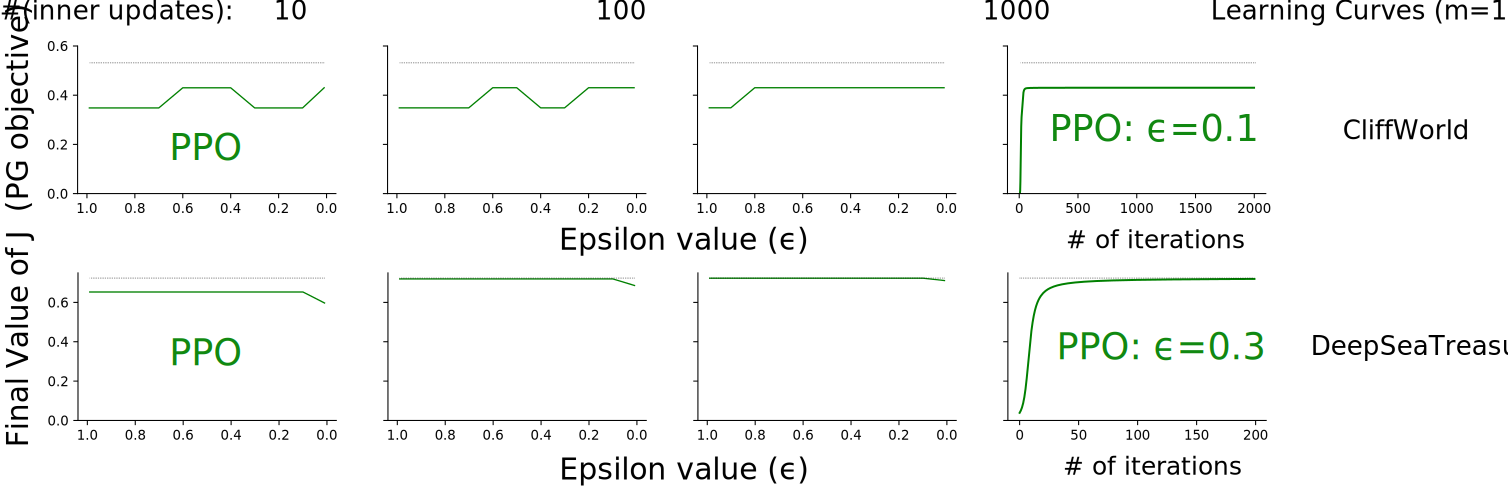
\includegraphics[width=0.9\textwidth]{ppo.pdf}
    \caption{The parameter sensitivity plots for the  PG algorithms on the CliffWorld environment for different number of inner loop updates. The $x$ axis shows sweep over one parameter of the corresponding PG algorithm. And for each point on the $x$-axis, we chose the best performing second parameter of the algorithm: the inner loop stepsize $\alpha$ for the first row, the Armijo constant for the second row, and there is no additional parameter for the last row. The faint black line near the top of each subplot depicts the value of the optimal policy.
    \label{fig:ppo_plots}}
\end{figure*}

\begin{figure*}[t]
    \centering
    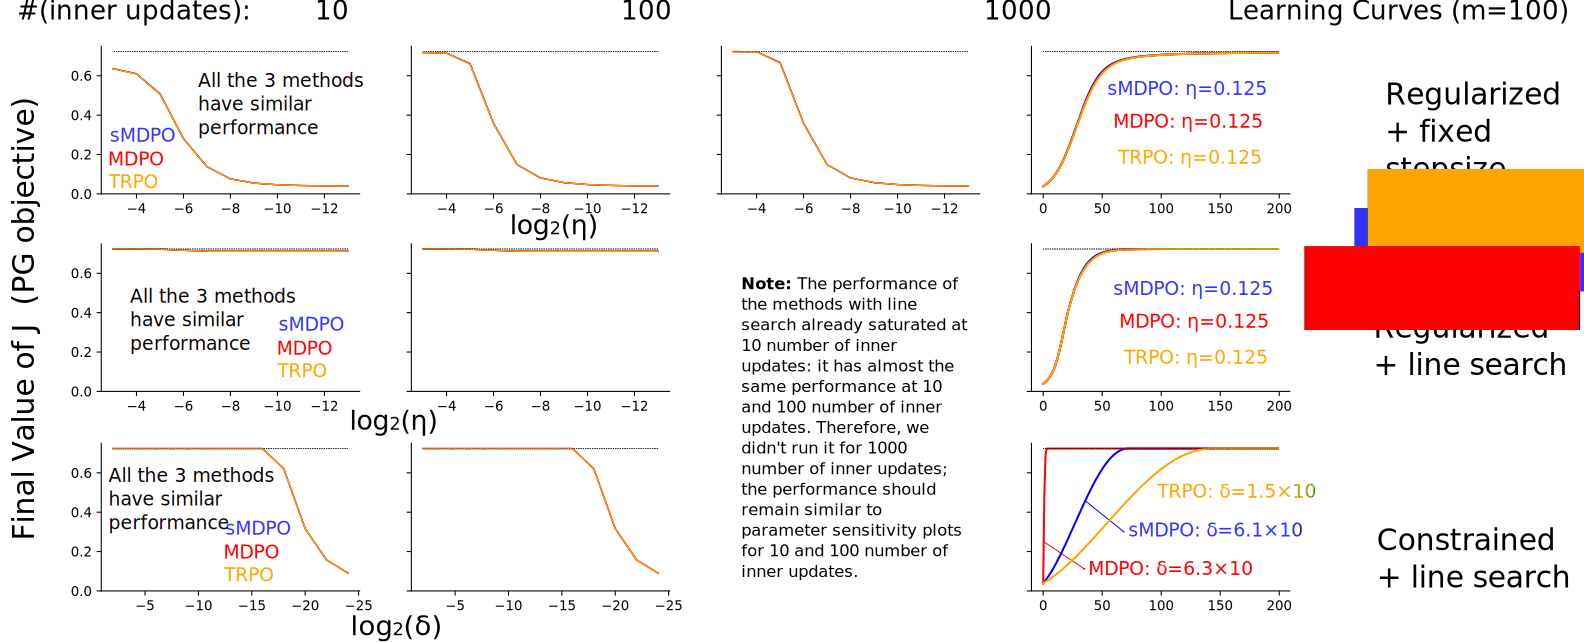
\includegraphics[width=0.9\textwidth]{deep_sea_treasure_ablation.pdf}
    \caption{The parameter sensitivity plots for the  PG algorithms on the CliffWorld environment for different number of inner loop updates. The $x$ axis shows sweep over one parameter of the corresponding PG algorithm. And for each point on the $x$-axis, we chose the best performing second parameter of the algorithm: the inner loop stepsize $\alpha$ for the first row, the Armijo constant for the second row, and there is no additional parameter for the last row. The faint black line near the top of each subplot depicts the value of the optimal policy.
    \label{fig:dst_sensitivity_plots}}
\end{figure*}

\subsection{Discussion} \sec{app:tabular_discussion}
The experiments for sMDPO served as a verification of the theoretical properties of the FMA-PG framework studied in this paper. We also compared it against other popular policy gradient algorithms from a pure optimization perspective. Our results demonstrated that sMDPO was competitive (or superior) to the popular PG methods. It was also somewhat robust to the hyperparameters; in particular we found that the algorithm, for all the value of $\eta$ suggested by theory, was able to converge to a locally optimal policy. The results also highlighted the importance of re-using data, i.e. doing multiple off-policy type of PG updates: as we increased the number of inner updates, the performance of all the methods seem to improve. They not only enjoyed faster convergence, but they also started to work for a wider range of parameters. This demonstrates the strength of these methods over simpler algorithms like REINFORCE \citep{williams1992simple} which only have a single update per batch of sampled data. To conclude, experiments with sMDPO suggest that the FMA-PG framework is a systematic way of obtaining new policy gradient algorithms that enjoy desirable theoretical properties and can be competitive to existing PG method, as suggested by our empirical results. We also include the self-contained code for these experiments with the submission.

\section{Analytical Updates and Gradient Expressions for tabular PG Algorithms} \label{app:tabular_derivations}
In the rest of this section, we give the calculations (the closed form analytical solutions for sMDPO and MDPO, and the gradient expressions for all four algorithms) employed in our implementation for tabular PG algorithms given in Appendix \ref{app:tabular_experiments}.

\subsection{sMDPO with Tabular Parameterization}
\subsubsection{Closed Form Update with Direct Representation}
Our goal is to find the closed form solution to the following optimization problem (from Eq. \ref{eq:fmd-softmax-kl-practical}, main paper):
\begin{equation}
  \pi_{t+1} = \arg\max_{\pi \in \Pi} \underbrace{\left[ \sum_s d^{\pi_t}(s) \sum_a p^{\pi_t}(a | s) \left(A^{\pi_t}(s, a) + \frac{1}{\eta} \right) \log \frac{p^\pi(s, a)}{p^{\pi_t}(s, a)} \right]}_{=: \ell^{\pi_t}_{\text{sMDPO}}}, \label{eq: optim_problem_sppo}
\end{equation}
subject to the constraints on policy $p^\pi$. We will solve this problem by assuming the policy $\pi \equiv p^\pi$ as an $|\mathcal{S}| \times |\mathcal{A}|$ table satisfying the standard constraints
\begin{align*}
  \sum_a p^\pi(a | s) &= 1,  \quad \forall s \in \mathcal{S} \\
  p^\pi(a | s) &\geq 0,  \quad \forall s \in \mathcal{S}, \; \forall a \in \mathcal{A}.
\end{align*}
We begin by formulating this problem using Lagrange multipliers $\{\lambda_s\}_{s \in \mathcal{S}}$ and $\{\lambda_{s, a}\}_{s, a \in \mathcal{S} \times \mathcal{A}}$ for all states $s$ and actions $a$:
\begin{align}
  \mathcal{L}(p^\pi, \lambda_s, \lambda_{s, a}) &= \sum_s d^{\pi_t}(s) \sum_a p^{\pi_t}(a | s) \left(A^{\pi_t}(s, a) + \frac{1}{\eta} \right) \log \frac{p^\pi(a | s)}{p^{\pi_t}(a | s)} \nonumber \\
  & \quad \; - \sum_{s, a} \lambda_{s, a} p^\pi(a | s) - \sum_s \lambda_{s} \bigg( \sum_a p^\pi(a | s) - 1 \bigg),
\end{align}
where we abused the notation, in $\mathcal{L}(p^\pi, \lambda_s, \lambda_{s, a})$, by using $\lambda_s$ to represent the set $\{\lambda_s\}_{s \in \mathcal{S}}$ and $\lambda_{s, a}$ to represent the set $\{\lambda_{s, a}\}_{s, a \in \mathcal{S} \times \mathcal{A}}$. The KKT conditions (Theorem 12.1, \citet{nocedal2006numerical}) for this constrained optimization problem can be written as:
\begin{align}
  \nabla_{p^\pi(b|x)} \mathcal{L}(p^\pi, \lambda_s, \lambda_{s, a}) &= 0, \quad \forall x \in \mathcal{S}, \; \forall b \in \mathcal{A} \tag{C1} \label{eq: KKT1} \\
  \sum_a p^\pi(a | s) &= 1, \quad \forall s \in \mathcal{S} \tag{C2} \label{eq: KKT2} \\
  p^\pi(a | s) &\geq 0, \quad \forall s \in \mathcal{S}, \; \forall a \in \mathcal{A} \tag{C3} \label{eq: KKT3} \\
  \lambda_s &\geq 0, \quad \forall s \in \mathcal{S} \tag{C4} \label{eq: KKT4} \\
  \lambda_{s} \bigg( \sum_a p^\pi(a | s) - 1 \bigg) &= 0, \quad \forall s \in \mathcal{S} \tag{C5} \label{eq: KKT5} \\
  \lambda_{s, a} p^\pi(a | s) &= 0, \quad \forall s \in \mathcal{S}, \; \forall a \in \mathcal{A}. \tag{C6} \label{eq: KKT6}
\end{align}

We now solve this system. Simplifying Eq. \ref{eq: KKT1} for an arbitrary state-action pair $(x, b)$ gives us:
\begin{align}
  \nabla_{p^\pi(b | x)} \mathcal{L}(p^\pi, \lambda_s, \lambda_{s, a}) &= d^{\pi_t}(x) p^{\pi_t}(b|x) \left( A^{\pi_t}(x, b) + \frac{1}{\eta} \right) \frac{1}{p^\pi(b|x)} - \lambda_{x, b} - \lambda_x = 0 \nonumber \\
  \Rightarrow \qquad \qquad \qquad \quad p^\pi(b | x) &= \frac{d^{\pi_t}(x) p^{\pi_t}(b|x) (1 + \eta A^{\pi_t}(x, b))}{\eta (\lambda_x + \lambda_{x, b})}. \label{eq: lagrangian_derivative_sppo}
\end{align}
Let us set 
\begin{equation}
  \lambda_{s, a} = 0, \quad \forall s \in \mathcal{S}, \; \forall a \in \mathcal{A}.
\end{equation}
Combining Eq. \ref{eq: lagrangian_derivative_sppo} with the second KKT condition gives us
\begin{equation}
  \lambda_s = \frac{1}{\eta} \sum_a d^{\pi_t}(s) p^{\pi_t}(a|s) (1 + \eta A^{\pi_t}(s, a)).
\end{equation}
Therefore, with the standard coverage assumption $d^{\pi_t}(s) > 0$, $p^\pi(a | s)$ becomes
\begin{equation}
  p^\pi(a | s) = \frac{p^{\pi_t}(a|s) (1 + \eta A^{\pi_t}(s, a))}{\sum_b p^{\pi_t}(b|s) (1 + \eta A^{\pi_t}(s, b))}.
\end{equation}
Note that $d^{\pi_t}(s), p^{\pi_t}(a|s) \geq 0$ for any state-action pair, since they are proper measures. We also need to ensure that
\begin{equation*}
  1 + \eta A^{\pi_t}(s, a) \geq 0
\end{equation*}
to satisfy the third and fourth KKT conditions. One straightforward way to achieve this is to define $p^\pi(a | s) = 0$ whenever $1 + \eta A^{\pi_t}(s, a) < 0$, and accordingly re-define $\lambda_s$. This gives us the final solution to our original optimization problem (Eq. \ref{eq: optim_problem_sppo}):
\begin{equation}
  \pi_{t+1} = p^\pi(s, a) = \frac{p^{\pi_t}(a|s) \max(1 + \eta A^{\pi_t}(s, a), 0)}{\sum_b p^{\pi_t}(b|s) \max(1 + \eta A^{\pi_t}(s, b), 0)}.
\end{equation}
However, it leaves us one last problem to deal with: Is it always true that given any state $s$, there always exists atleast one action $a$, such that $1 + \eta A^{\pi_t}(s, a) \geq 0$? Because otherwise, we would fail to satisfy the second KKT condition. But not that this is not a problem since we can put a condition on $\eta$ in order to fulfill this constraint.

\subsubsection{Gradient of the Loss Function with Softmax Policy Representation}
Consider the softmax policy representation
\begin{equation}
  p^\pi(b | x) = \frac{e^{\theta(x, b)}}{\sum_c e^{\theta(x, c)}}, \label{eq: softmax}
\end{equation}
where $\theta(x, b)$ for all state-action pairs $(x, b)$ are action preferences maintained in a table (tabular parameterization). Also note that the derivative of the policy with respect to the action preferences is given by
\begin{equation}
  \frac{\partial}{\partial \theta(s, a)} p^\pi(b | x) = \mathbb{I}(x = s) \Big( \mathbb{I}(b = a) - p^\pi(a | x) \Big) p^\pi(b | x),
\end{equation}
where $\mathbb{I}(a = b)$ is the identity function when $a = b$ and zero otherwise. 
We will use gradient ascent to approximately solve Eq. \ref{eq: optim_problem_sppo}; to do that, the quantity of interest is
\begin{align}
  \frac{\partial}{\partial \theta(s, a)} \ell^{\pi_t}_{\text{sMDPO}} &= \sum_{x \in \mathcal{S}} \sum_{b \in \mathcal{A}} \left[ \frac{\partial}{\partial \theta(s, a)} p^\pi(b | x) \right] \left[ \frac{\partial}{\partial p^\pi(b | x)} \ell^{\pi_t}_{\text{sMDPO}} \right] \tag*{(using total derivative)} \\
  &= \sum_{x, b} \Big[ \mathbb{I}(x = s) \Big( \mathbb{I}(b = a) - p^\pi(a | x) \Big) p^\pi(b | x) \Big] \left[ d^{\pi_t}(x) p^{\pi_t}(b|x) \left( A^{\pi_t}(x, b) + \frac{1}{\eta} \right) \frac{1}{p^\pi(b|x)} \right] \nonumber \\
  &= \E_{X \sim d^{\pi_t}, B \sim p^{\pi_t}(\cdot | X)} \left[ \mathbb{I}(X = s) \Big( \mathbb{I}(B = a) - p^\pi(a | x) \Big) \left( A^{\pi_t}(X, B) + \frac{1}{\eta} \right) \right] \\
  &= d^{\pi_t}(s) \sum_b \Big( \mathbb{I}(b = a) - p^\pi(a | s) \Big) p^{\pi_t}(b|s) \left( A^{\pi_t}(s, b) + \frac{1}{\eta} \right) \nonumber \\
  &= d^{\pi_t}(s) \left[ p^{\pi_t}(a|s) \left( A^{\pi_t}(s, a) + \frac{1}{\eta} \right) - p^\pi(a | s) \sum_b p^{\pi_t}(b|s) \left(A^{\pi_t}(s, b) + \frac{1}{\eta} \right) \right] \nonumber \\
  &= d^{\pi_t}(s) \left[ p^{\pi_t}(a|s) \left( A^{\pi_t}(s, a) + \frac{1}{\eta} \right) - \frac{p^\pi(a | s)}{\eta} \right], \nonumber
\end{align}
Now we can simply update the inner loop of FMA-PG (Algorithm 1, main paper) via gradient ascent:
\begin{equation}
  \theta(s, a) \; \leftarrow \; \theta(s, a) + \alpha d^{\pi_t}(s) \left[ p^{\pi_t}(a|s) \left( A^{\pi_t}(s, a) + \frac{1}{\eta} \right) - \frac{p^\pi(a | s)}{\eta} \right].
\end{equation}

\subsection{Mirror Descent Policy Optimization (MDPO)}
In this section, we study the MDPO type FMA-PG update (Eq. \ref{eq:fmd-softmax-statewise} in main paper). We first calculate the analytical solution to that optimization problem, and then calculate its gradient which we use in the experiments. However, in the analysis that follows, we we replace the advantage function $A^{\pi_t}$ with the action-value function $Q^{\pi_t}$ to make it exactly same as the original MDPO \citep{tomar2020mirror} update.
\subsubsection{Closed Form Update with Direct Parameterization}
While giving the MDPO type FMA-PG equation (Eq. \ref{eq:fmd-softmax-statewise}), the paper considers the direct representation along with tabular parameterization of the policy, albeit with a small change in notation as compared to the previous subsection: $\pi(a|s) \equiv p^\pi(a|s, \theta)$. However, since this notation is more cumbersome, we will stick with our the notation of the previous subsection: $\pi(a|s) \equiv p^\pi(a|s)$. The constraints on the parameters $p^\pi(s, a)$ are the same as before: $\sum_a p^\pi(a | s) = 1, \; \forall s \in \mathcal{S}$; and $p^\pi(a | s) \geq 0, \; \forall s \in \mathcal{S}, \; \forall a \in \mathcal{A}$. Our goal, this time, is to solve the following optimization problem (from Eq. 6, main paper)
\begin{equation}
  \pi_{t+1} = \arg\max_{\pi \in \Pi} \underbrace{\left[ \sum_s d^{\pi_t}(s) \sum_a p^{\pi_t}(a|s) \left( Q^{\pi_t}(s, a) \frac{p^\pi(a | s)}{p^{\pi_t}(a | s)} - \frac{1}{\eta} D_\phi (p^\pi(\cdot | s), p^{\pi_t}(\cdot | s)) \right) \right]}_{=: \ell^{\pi_t}_{\text{MDPO}}}, \label{eq: optim_problem_mdpo}
\end{equation}
with the mirror map as the negative entropy (Eq. 5.27, \citet{beck2003mirror}). This particular choice of the mirror map simplifies the Bregman divergence as follows
\begin{equation}
  D_\phi (p^\pi(\cdot | s), p^{\pi_t}(\cdot | s)) = \text{KL}(p^\pi(\cdot | s) \| p^{\pi_t}(\cdot | s)) := \sum_a p^\pi(a | s) \log \frac{p^\pi(a | s)}{p^{\pi_t}(a | s)}.
\end{equation}
The optimization problem (Eq. \ref{eq: optim_problem_mdpo}) then simplifies to
\begin{equation}
  \pi_{t+1} = \arg\max_{\pi \in \Pi} \left[ \sum_s d^{\pi_t}(s) \sum_a p^{\pi_t}(a|s) \left( Q^{\pi_t}(s, a) \frac{p^\pi(a | s)}{p^{\pi_t}(a | s)} - \frac{1}{\eta} \sum_{a'} p^\pi(a' | s) \log \frac{p^\pi(a' | s)}{p^{\pi_t}(a' | s)} \right) \right].
\end{equation}

Proceeding analogously to the previous subsection, we use Lagrange multipliers $\lambda_s$, $\lambda_{s, a}$ for all states $s$ and actions $a$ to obtain the function
\begin{align}
  \mathcal{L}(p^\pi, \lambda_s, \lambda_{s, a}) &= \sum_s d^{\pi_t}(s) \sum_a p^{\pi_t}(a|s) Q^{\pi_t}(s, a) \frac{p^\pi(a | s)}{p^{\pi_t}(a | s)} - \frac{1}{\eta} \sum_s d^{\pi_t}(s) \sum_{a'} p^\pi(a' | s) \log \frac{p^\pi(a' | s)}{p^{\pi_t}(a' | s)} \nonumber \\
  & \quad \; - \sum_{s, a} \lambda_{s, a} p^\pi(a | s) - \sum_s \lambda_{s} \bigg( \sum_a p^\pi(a | s) - 1 \bigg).
\end{align}
The KKT conditions are exactly the same as before (Eq. \ref{eq: KKT1} to Eq. \ref{eq: KKT6}).

Again, we begin by solving the first KKT condition:
\begin{align}
  \nabla_{p^\pi(b | x)} \mathcal{L}(p^\pi, \lambda_s, \lambda_{s, a}) &= d^{\pi_t}(x) p^{\pi_t}(b|x) \frac{Q^{\pi_t}(x, b)}{p^{\pi_t}(b | x)} - \frac{d^{\pi_t}(x)}{\eta} \left[ \log \frac{p^\pi(b | x)}{p^{\pi_t}(b | x)} + 1 \right] - \lambda_{x, b} - \lambda_x \nonumber \\
  &= \frac{d^{\pi_t}(x)}{\eta} \left[ \eta Q^{\pi_t}(x, b) - \log \frac{p^\pi(b | x)}{p^{\pi_t}(b | x)} - 1 - \frac{\eta (\lambda_{x, b} + \lambda_x)}{d^{\pi_t}(x)} \right] \nonumber \\
  &= 0 \nonumber \\
  \Rightarrow \qquad \qquad \log \frac{p^\pi(b | x)}{p^{\pi_t}(b | x)} &= \eta Q^{\pi_t}(x, b) - \frac{\eta (\lambda_{x, b} + \lambda_x)}{d^{\pi_t}(x)} - 1 \nonumber \\
  \Rightarrow \qquad \qquad \qquad p^\pi(b | x) &= p^{\pi_t}(b | x) \cdot e^{\eta Q^{\pi_t}(x, b)} \cdot e^{- \frac{\eta (\lambda_{x, b} + \lambda_x)}{d^{\pi_t}(x)} - 1}, \label{eq: lagrangian_derivative_mdpo}
\end{align}
where in the fourth line, we used the assumption that $d^{\pi_t}(x) > 0$ for all states $x$. We again set
\begin{equation}
  \lambda_{s, a} = 0, \quad \forall s \in \mathcal{S}, \; \forall a \in \mathcal{A}.
\end{equation}
And, we put Eq. \ref{eq: lagrangian_derivative_mdpo} in the second KKT condition to get
\begin{equation}
  e^{- \frac{\eta \lambda_x}{d^{\pi_t}(x)} - 1} = \left( \sum_b p^{\pi_t}(b | x) \cdot e^{\eta Q^{\pi_t}(x, b)} \right)^{-1}.
\end{equation}
Therefore, we obtain
\begin{equation}
  p^\pi(a | s) = \frac{p^{\pi_t}(a | s) \cdot e^{\eta Q^{\pi_t}(s, a)}}{\sum_b p^{\pi_t}(b | s) \cdot e^{\eta Q^{\pi_t}(s, b)}}.
\end{equation}
This leaves one last problem: Can we ensure that $\lambda_s \geq 0$ for all states $s$? If not, then the fourth KKT condition cannot be satisfied. Again, we can set the stepsize $\eta$ in such a way, such that this constraint is always fulfilled.

\subsubsection{Gradient of the MDPO Loss Function with Tabular Softmax Representation}
We again take the softmax policy representation given by Eq. \ref{eq: softmax}, and compute $\nabla_{\theta(s, a)} \ell^{\pi_t}_{\text{MDPO}}$ for the MDPO loss (we substitute $Q^{\pi_t}$ with $A^{\pi_t}$ in this calculation):
\begin{align}
  \frac{\partial}{\partial \theta(s, a)} \ell^{\pi_t}_{\text{MDPO}} &= \sum_{x, b} \left[ \frac{\partial}{\partial \theta(s, a)} p^\pi(b | x) \right] \left[ \frac{\partial}{\partial p^\pi(b | x)} \ell^{\pi_t}_{\text{MDPO}} \right] \tag*{(using total derivative)} \\
  &= \sum_{x, b} \Big[ \mathbb{I}(x = s) \Big( \mathbb{I}(b = a) - p^\pi(a | x) \Big) p^\pi(b | x) \Big] \left[ \frac{d^{\pi_t}(x)}{\eta} \left( \eta A^{\pi_t}(x, b) - \log \frac{p^\pi(b | x)}{p^{\pi_t}(b | x)} - 1 \right) \right] \nonumber \\
  &= \frac{d^{\pi_t}(s)}{\eta} \sum_b \Big( \mathbb{I}(b = a) - p^\pi(a | s) \Big) p^\pi(b | s) \left[ \eta A^{\pi_t}(s, b) - \log \frac{p^\pi(b | s)}{p^{\pi_t}(b | s)} - 1 \right] \nonumber \\
  &= \frac{d^{\pi_t}(s)}{\eta} p^\pi(a | s) \left[ \eta A^{\pi_t}(s, a) - \eta \sum_b p^\pi(b|s) A^{\pi_t}(s, b) - \log \frac{p^\pi(a | s)}{p^{\pi_t}(a | s)} + \text{KL}(p^\pi(\cdot | s) \| p^{\pi_t}(\cdot | s)) \right], \nonumber
\end{align}
where in the last line, we used the fact that
\begin{equation*}
  \sum_b p^\pi(b | s) \left[ \eta A^{\pi_t}(s, b) - \log \frac{p^\pi(b | s)}{p^{\pi_t}(b | s)} - 1 \right] = \eta \sum_b p^\pi(b|s) A^{\pi_t}(s, b) - \text{KL}(p^\pi(\cdot | s) \| p^{\pi_t}(\cdot | s)) - 1.
\end{equation*}

\subsection{Trust Region Policy Optimization (TRPO)}
At each step of the policy update, TRPO (Eq. 14, \citet{schulman2015trust}) solves the following problem:
\begin{equation}
  \max_\theta \; \underbrace{\sum_s d^{\pi_t}(s) \sum_a p^{\pi_\theta}(a | s) Q^{\pi_t}(s, a)}_{=: \mathcal{J}_{\text{TRPO}}} \qquad \text{subject to } \underbrace{\sum_s d^{\pi_t}(s) \cdot \text{KL}(p^{\pi_t}(\cdot | s) \| p^{\pi_\theta}(\cdot | s))}_{=: \mathcal{C}_{\text{TRPO}}} \leq \delta.  
\end{equation}
Unlike the sMDPO and the MDPO updates, an analytical solution cannot be derived for this update (since it would require solving a system of non-trivial non-linear equations). Therefore, we will use gradient based methods to approximately solve this problem. From Appendix C of \citet{schulman2015trust}, the descent direction is given by $s \approx A^{-1} g$ where the vector $g$ is defined as $g_{(s, a)} := \frac{\partial}{\partial \theta(s, a)} \mathcal{J}_{\text{TRPO}}$, and the matrix $A$ is defined as $A_{(s, a), (s', a')} := \frac{\partial}{\partial \theta(s, a)} \frac{\partial}{\partial \theta(s', a')} \mathcal{C}_{\text{TRPO}}$. We analytically compute the expression for this direction assuming a softmax policy (Eq. \ref{eq: softmax}). The vector $g$ can be readily calculated as
\begin{align}
  \frac{\partial}{\partial \theta(s, a)} \mathcal{J}_{\text{TRPO}} &= \sum_x d^{\pi_t}(x) \sum_b Q^{\pi_t}(x, b) \frac{\partial p^{\pi_\theta}(b | x)}{\partial \theta(s, a)} \nonumber \\
  &= \sum_x d^{\pi_t}(x) \sum_b Q^{\pi_t}(x, b) \mathbb{I}(x = s) \Big( \mathbb{I}(b = a) - p^{\pi_\theta}(a | x) \Big) p^{\pi_\theta}(b | x) \nonumber \\
  &= \sum_x d^{\pi_t}(x) \mathbb{I}(x = s) \left[ \sum_b \mathbb{I}(b = a) p^{\pi_\theta}(b | x) Q^{\pi_t}(x, b) - p^{\pi_\theta}(a | x) \sum_b p^{\pi_\theta}(b | x) Q^{\pi_t}(x, b) \right] \nonumber \\
  &= d^{\pi_t}(s) p^{\pi_\theta}(a | s) \left[ Q^{\pi_t}(s, a) - \sum_b p^{\pi_\theta}(b | s) Q^{\pi_t}(s, b) \right]. \label{eq: trpo_gradient}
\end{align}
For calculating the matrix $A$, we use the law of total derivative to obtain
\begin{align}
  \frac{\partial}{\partial \theta(s, a)} \mathcal{C}_{\text{TRPO}} &= \sum_{x, b} \left[ \frac{\partial}{\partial \theta(s, a)} p^{\pi_\theta}(b | x) \right] \left[ \frac{\partial}{\partial p^{\pi_\theta}(b | x)} \sum_s d^{\pi_t}(s) \sum_a p^{\pi_t}(a | s) \log \frac{p^{\pi_t}(a | s)}{p^{\pi_\theta}(a | s)} \right] \nonumber \\
  &= \sum_{x, b} \left[ \mathbb{I}(x = s) \Big( \mathbb{I}(b = a) - p^{\pi_\theta}(a | x) \Big) p^{\pi_\theta}(b | x) \right] \left[ - d^{\pi_t}(x) \frac{p^{\pi_t}(b | x)}{p^{\pi_\theta}(b | x)} \right] \nonumber \\
  &= - d^{\pi_t}(s) \sum_b \Big( \mathbb{I}(b = a) - p^{\pi_\theta}(a | s) \Big) p^{\pi_t}(b | s) \nonumber \\
  &= - d^{\pi_t}(s) \left[ \sum_b \mathbb{I}(b = a) p^{\pi_t}(b | s) - p^{\pi_\theta}(a | s) \sum_b p^{\pi_t}(b | s) \right] \nonumber \\
  &= d^{\pi_t}(s) \Big[ p^{\pi_\theta}(a | s) - p^{\pi_t}(a | s) \Big]. \label{eq: trpo_kl_mid}
\end{align}
Finally, using the above result yields
\begin{align}
  \frac{\partial}{\partial \theta(s, a)} \frac{\partial}{\partial \theta(s', a')} \mathcal{C}_{\text{TRPO}} &= \frac{\partial}{\partial \theta(s, a)} d^{\pi_t}(s') \Big[ p^{\pi_\theta}(a' | s') - p^{\pi_t}(a' | s') \Big] \nonumber \\
  &= d^{\pi_t}(s') \cdot \frac{\partial}{\partial \theta(s, a)} p^{\pi_\theta}(a' | s') \nonumber \\
  &= \mathbb{I}(s'=s) \cdot d^{\pi_t}(s') \Big( \mathbb{I}(a'=a) - p^{\pi_\theta}(a | s') \Big) p^{\pi_\theta}(a' | s') \\
  \Rightarrow \qquad \qquad \qquad \quad A_{(s, :), (s, :)} &= d^{\pi_t}(s) \Big( \text{diag} (p^{\pi_\theta}(\cdot | s)) - p^{\pi_\theta}(\cdot | s) p^{\pi_\theta}(\cdot | s)^\top \Big),
\end{align}
where $p^{\pi_\theta}(\cdot | s) \in \mathbb{R}^{|\mathcal{A}|}$ is the vector defined as $[p^{\pi_\theta}(\cdot | s)]_a = p^{\pi_\theta}(a | s)$ and $A_{(s, :), (s, :)}$ denotes the square sub-block of the matrix $A$ corresponding to the given state $s$ and all the actions. In our experiments, since our $A$ matrix is small, we directly take its inverse to compute the update direction, thereby bypassing the conjugate method. Once we have the update direction, we then compute the maximal stepsize $\beta$ and perform an exponential backtracking line search as explained in the TRPO paper.

\subsection{Proximal Policy Optimization (PPO)}
The Proximal Policy Optimization algorithm \citep{schulman2017proximal} solves the following optimization problem at each iteration step:
\begin{equation}
  \max_\theta \; \underbrace{\sum_s d^{\pi_t}(s) \sum_a p^{\pi_t}(a | s) \cdot \min \left( \begin{matrix} \frac{p^{\pi_\theta}(a | s)}{p^{\pi_t}(a | s)} A^{\pi_t}(s, a), \\ \text{clip} \left[\frac{p^{\pi_\theta}(a | s)}{p^{\pi_t}(a | s)}, 1 - \epsilon, 1 + \epsilon \right] A^{\pi_t}(s, a) \end{matrix} \right)}_{=: \mathcal{J}_{\text{PPO}}}.
\end{equation}
The gradient of the objective $\mathcal{J}_{\text{PPO}}$ can be shown to be equivalent to
\begin{equation}
  \nabla \mathcal{J}_{\text{PPO}} = \sum_s d^{\pi_t}(s) \sum_a p^{\pi_t}(a | s) \cdot \mathbb{I} \Big( \text{cond}(s, a) \Big) \frac{\nabla p^{\pi_\theta}(a | s)}{p^{\pi_t}(a | s)} A^{\pi_t}(s, a),
\end{equation}
where 
\begin{equation}
  \text{cond}(s, a) = \left( A^{\pi_t}(s, a) > 0 \;\bigwedge\; \frac{p^{\pi_\theta}(a | s)}{p^{\pi_t}(a | s)} < 1 + \epsilon \right) \;\bigvee\; \left( A^{\pi_t}(s, a) < 0 \;\bigwedge\; \frac{p^{\pi_\theta}(a | s)}{p^{\pi_t}(a | s)} > 1 - \epsilon \right).
\end{equation}
Repeating our usual drill, we assume a softmax policy to obtain:
\begin{align}
  & \frac{\partial}{\partial \theta(s, a)} \mathcal{J}_{\text{PPO}} \nonumber \\
  &= \sum_x d^{\pi_t}(x) \sum_b \mathbb{I} \Big( \text{cond}(x, b) \Big) \frac{\partial p^{\pi_\theta}(b | x)}{\partial \theta(s, a)} A^{\pi_t}(x, b) \nonumber \\
  &= \sum_x d^{\pi_t}(x) \sum_b \mathbb{I} \Big( \text{cond}(x, b) \Big) \mathbb{I}(x = s) \Big( \mathbb{I}(b = a) - p^{\pi_\theta}(a | x) \Big) p^{\pi_\theta}(b | x) A^{\pi_t}(x, b) \nonumber \\
  &= d^{\pi_t}(s) \Bigg[ \sum_b \mathbb{I}(b = a) \mathbb{I} \Big( \text{cond}(s, b) \Big) p^{\pi_\theta}(b | s) A^{\pi_t}(s, b) - p^{\pi_\theta}(a | s) \sum_b \mathbb{I} \Big( \text{cond}(s, b) \Big) p^{\pi_\theta}(b | s) A^{\pi_t}(s, b) \Bigg] \nonumber \\
    &= d^{\pi_t}(s) p^{\pi_\theta}(a | s) \left[ \mathbb{I} \Big( \text{cond}(s, a) \Big) A^{\pi_t}(s, a) - \sum_b p^{\pi_\theta}(b | s) \mathbb{I} \Big( \text{cond}(s, b) \Big) A^{\pi_t}(s, b) \right]. \label{eq: ppo_gradient}
\end{align}
The PPO gradient (Eq. \ref{eq: ppo_gradient}) is exactly the same as the TRPO gradient (Eq. \ref{eq: trpo_gradient}) except for the additional condition on choosing only specific state-action pairs while calculating the difference between advantage under the current policy and the approximate change in advantage under the updated policy.

\subsection{MDPO with Constraints}
In this section, we calculate the second derivative of the MDPO constraint as given in Table \ref{table: ablation_study}. This will allow us compute the Hessian $A^{\text{MDPO}}$, which is the analog of the $A$ matrix from TRPO implementation, and help us implement MDPO with a constrained objective and line search.

Continuing from the gradient of the MDPO constraint given in Table \ref{table: ablation_study_grad}, we get
\begin{align}
  \frac{\partial}{\partial p^\pi(b | x)} \frac{\partial \mathcal{C}_{\text{MDPO}}}{\partial \theta(s', a')} &= \frac{\partial}{\partial p^\pi(b | x)} d^{\pi_t}(s') p^\pi(a' | s') \left( \log \frac{p^\pi(a' | s')}{p^{\pi_t}(a' | s')} - \sum_c p^\pi(c | s') \log \frac{p^\pi(c | s')}{p^{\pi_t}(c | s')} \right) \nonumber \\
  &= \mathbb{I}(x = s') d^{\pi_t}(s') \Bigg[ \mathbb{I}(b = a') \left( \log \frac{p^\pi(a' | s')}{p^{\pi_t}(a' | s')} - \sum_c p^\pi(c | s') \log \frac{p^\pi(c | s')}{p^{\pi_t}(c | s')} \right) \nonumber \\
    & \qquad \qquad \qquad \qquad \quad + p^\pi(a' | s') \frac{\mathbb{I}(b = a')}{p^\pi(a' | s')} - p^\pi(a' | s') \left( \log \frac{p^\pi(b | s')}{p^{\pi_t}(b | s')} + 1 \right) \Bigg] \nonumber \\
  &= \mathbb{I}(x = s') d^{\pi_t}(s') \Bigg[ \mathbb{I}(b = a') \cdot T_{\text{itd}}(s', a') - p^\pi(a' | s') \left( \log \frac{p^\pi(b | s')}{p^{\pi_t}(b | s')} + 1 \right) \Bigg],
\end{align}
where we introduced an intermediate variable $T_{\text{itd}}(s', a') := \log \frac{p^\pi(a' | s')}{p^{\pi_t}(a' | s')} - \text{KL} ( p^\pi(\cdot | s') \| p^{\pi_t}(\cdot | s') ) + 1$. Now, using the law of total derivative, we obtain
\begin{align}
  \frac{\partial}{\partial \theta(s, a)} \frac{\partial \mathcal{C}_{\text{MDPO}}}{\partial \theta(s', a')} &= \sum_{x, b} \frac{\partial p^\pi(b | x)}{\partial \theta(s, a)} \times \frac{\partial}{\partial p^\pi(b | x)} \frac{\partial \mathcal{C}_{\text{MDPO}}}{\partial \theta(s', a')} \nonumber \\
  &= \sum_{x, b} \mathbb{I}(x = s) \Big[ \mathbb{I}(b = a) - p^\pi(a | x) \Big] p^\pi(b | x) \times \mathbb{I}(x = s') d^{\pi_t}(s') \nonumber \\
  & \qquad \quad \times \Bigg[ \mathbb{I}(b = a') \cdot T_{\text{itd}}(s', a') - p^\pi(a' | s') \left( \log \frac{p^\pi(b | s')}{p^{\pi_t}(b | s')} + 1 \right) \Bigg] \nonumber \\
  &= \mathbb{I}(s = s') d^{\pi_t}(s) \cdot T_{\text{aux}},
\end{align}
where the auxillary term $T_{\text{aux}}$ is 
\begin{align}
  T_{\text{aux}} &:= \sum_b \Big[ \mathbb{I}(b = a) - p^\pi(a | s) \Big] p^\pi(b | s) \Bigg[ \mathbb{I}(b = a') \cdot T_{\text{itd}}(s, a') - p^\pi(a' | s) \left( \log \frac{p^\pi(b | s)}{p^{\pi_t}(b | s)} + 1 \right) \Bigg] \\
  &= T_{\text{itd}}(s, a') \sum_{b} \mathbb{I}(b = a) p^\pi(b | s) \mathbb{I}(b = a') - p^\pi(a' | s) \sum_{b} \mathbb{I}(b = a) p^\pi(b | s) \left( \log \frac{p^\pi(b | s)}{p^{\pi_t}(b | s)} + 1 \right) \nonumber \\
  & \qquad - p^\pi(a | s) T_{\text{itd}}(s, a') \sum_{b} p^\pi(b | s) \mathbb{I}(b = a') + p^\pi(a' | s) p^\pi(a | s) \sum_{b} p^\pi(b | s) \left( \log \frac{p^\pi(b | s)}{p^{\pi_t}(b | s)} + 1 \right) \nonumber \\  
  &= T_{\text{itd}}(s, a') p^\pi(a | s) \mathbb{I}(a = a') - p^\pi(a' | s) p^\pi(a | s) \left( \log \frac{p^\pi(a | s)}{p^{\pi_t}(a | s)} + 1 \right) \nonumber \\
  & \qquad - p^\pi(a | s) T_{\text{itd}}(s, a') p^\pi(a' | s) + p^\pi(a' | s) p^\pi(a | s) \Big( \text{KL}( p^\pi(\cdot | s) \| p^{\pi_t}(\cdot | s) ) + 1 \Big) \nonumber \\
  &= \mathbb{I}(a = a') p^\pi(a | s) T_{\text{itd}}(s, a') - p^\pi(a' | s) p^\pi(a | s) \Big[ T_{\text{itd}}(s, a') + T_{\text{itd}}(s, a) \Big] + p^\pi(a' | s) p^\pi(a | s).
\end{align}
Therefore, 
\begin{align}
  \frac{\partial}{\partial \theta(s, a)} \frac{\partial \mathcal{C}_{\text{MDPO}}}{\partial \theta(s', a')} &= \mathbb{I}(s = s') d^{\pi_t}(s) \bigg[ \mathbb{I}(a = a') p^\pi(a | s) T_{\text{itd}}(s, a') - p^\pi(a | s) p^\pi(a' | s) T_{\text{itd}}(s, a') \nonumber \\
    & \qquad \qquad \qquad \qquad \quad - p^\pi(a' | s) p^\pi(a | s) T_{\text{itd}}(s, a) + p^\pi(a' | s) p^\pi(a | s) \bigg] \\
  \Rightarrow \qquad \qquad A^{\text{MDPO}}_{(s, :), (s, :)} &= d^{\pi_t}(s) \cdot \Big[ \text{diag} \big( T_{\text{vec}}(s) \big) - p^{\pi}(\cdot | s) T_{\text{vec}}(s)^\top \nonumber \\
    & \qquad \qquad \qquad - T_{\text{vec}}(s) p^{\pi}(\cdot | s)^\top + p^{\pi}(\cdot | s) p^{\pi}(\cdot | s)^\top \Big],
\end{align}
where we introduced yet another intermediate term $T_{\text{vec}}(s)$, defined as
\begin{align}
  T_{\text{vec}}(s) &:= p^{\pi}(\cdot | s) \odot T_{\text{itd}}(s, \cdot) \\
  &= p^{\pi}(\cdot | s) \odot \left[ \log \Big( p^\pi(\cdot | s) \oslash p^{\pi_t}(\cdot | s) \Big) - \text{KL} (p^\pi(\cdot | s) \| p^{\pi_t}(\cdot | s)) \mathbf{1}_{|\mathcal{A}|} + \mathbf{1}_{|\mathcal{A}|} \right],
\end{align}
and $\oslash$ in the above equation represents the elementwise vector division defined as $[a \oslash b]_i := a_i / b_i$ for any two vectors $a$ and $b$. As a sanity check, note that the matrix $A^{\text{MDPO}}$ is symmetric, as any Hessian matrix should be.


\section*{References}

\medskip
\small
\begin{list}{}{%
    \setlength{\topsep}{0pt}%
    \setlength{\leftmargin}{0.2in}%
    \setlength{\listparindent}{-0.2in}%
    \setlength{\itemindent}{-0.2in}%
    \setlength{\parsep}{\parskip}%
  }%

\item[] Beck, A., Teboulle, M. (2003). Mirror descent and nonlinear projected subgradient methods for convex optimization. \textit{Operations Research Letters, 31}(3), 167-175.

\item[] Nocedal, J., Wright, S. (2006). Numerical optimization. \textit{Springer Science \& Business Media.}

\item[] Schulman, J., Wolski, F., Dhariwal, P., Radford, A., Klimov, O. (2017). Proximal policy optimization algorithms. \textit{arXiv preprint arXiv:1707.06347.}

\item[] Schulman, J., Levine, S., Abbeel, P., Jordan, M., Moritz, P. (2015, June). Trust region policy optimization. In \textit{International conference on machine learning} (pp. 1889-1897). PMLR.

  \item[] Tomar, M., Shani, L., Efroni, Y., Ghavamzadeh, M. (2020). Mirror descent policy optimization. \textit{arXiv preprint arXiv:2005.09814.}
  
  \item[] Vaswani, S., Bachem, O., Totaro, S., Mueller, R., Geist, M., Machado, M. C., Castro P. S., Roux, N. L. (2021). A functional mirror ascent view of policy gradient methods with function approximation. \textit{arXiv preprint arXiv:2108.05828.}

\item[] Williams, R. J. (1992). Simple statistical gradient-following algorithms for connectionist reinforcement learning. \textit{Machine learning, 8}(3), 229-256.
  
\end{list}

\end{document}
